% This is LLNCS.DEM the demonstration file of
% the LaTeX macro package from Springer-Verlag
% for Lecture Notes in Computer Science,
% version 2.4 for LaTeX2e as of 16. April 2010
%
\documentclass{llncs}
%

% %% Save the class definition of \subparagraph
% \let\llncssubparagraph\subparagraph
% %% Provide a definition to \subparagraph to keep titlesec happy
% \let\subparagraph\paragraph
% %% Load titlesec
% \usepackage[compact]{titlesec}
% %% Revert \subparagraph to the llncs definition
% \let\subparagraph\llncssubparagraph
\usepackage{makeidx}  % allows for indexgeneration
\usepackage{url}
\usepackage{todonotes}
\usepackage{listings}
% \usepackage{bcprules}
\usepackage{fontspec}
\usepackage{fancyvrb}
\usepackage{mathpartir}
\usepackage[labelfont=bf]{caption}
\usepackage{subcaption}
\captionsetup{compatibility=false}
\usepackage[bottom]{footmisc}
\usepackage{longtable}
\usepackage{booktabs}
% \usepackage{pdflscape}
\usepackage{colortbl}%
  \newcommand{\myrowcolour}{\rowcolor[gray]{0.925}}
\usepackage{wasysym}

\usepackage{microtype}
\usepackage{times}
\usepackage[english]{babel}
\usepackage{graphicx}
\usepackage{xcolor}
\usepackage{lipsum}

% Member sequences
\newcommand{\seq}[1]{\overline{#1}}

% arrays
\newcommand{\ba}{\begin{array}}
\newcommand{\ea}{\end{array}}
\newcommand{\bda}{\[\ba}
\newcommand{\eda}{\ea\]}
\newcommand{\ei}{\end{array}}
\newcommand{\bcases}{\left\{\begin{array}{ll}}
\newcommand{\ecases}{\end{array}\right.}
\newcommand{\sporeurl}{\url{https://github.com/scala/spores}}
% spacing
\newcommand{\gap}{\quad\quad}
\newcommand{\andalso}{\quad\quad}
\newcommand{\biggap}{\quad\quad\quad}
\newcommand{\nextline}{\\ \\}
\newcommand{\htabwidth}{0.5cm}
\newcommand{\tabwidth}{1cm}
\newcommand{\htab}{\hspace{\htabwidth}}
\newcommand{\tab}{\hspace{\tabwidth}}
\newcommand{\linesep}{\ \hrulefill \ \smallskip}

\newcommand{\ie}{{\em i.e.,~}}
\newcommand{\eg}{{\em e.g.,~}}
\newcommand{\etc}{{\em etc}}

\lstdefinelanguage{Scala}%
{morekeywords={abstract,case,catch,char,class,%
    def,else,extends,final,%
    if,import,%
    match,module,new,null,object,override,package,private,protected,%
    public,return,super,this,throw,trait,try,type,val,var,with,implicit,%
    macro,sealed,%
  },%
  sensitive,%
  morecomment=[l]//,%
  morecomment=[s]{/*}{*/},%
  morestring=[b]",%
  morestring=[b]',%
  showstringspaces=false%
}[keywords,comments,strings]%

% \lstset{language=Scala,%
%   mathescape=true,%
%   columns=[c]fixed,%
%   numbers=left, numberstyle=\scriptsize\color{gray}\ttfamily,
%   basewidth={0.5em, 0.40em},%
%   basicstyle=\tt,%
%   xleftmargin=0.0cm
% }

\setmainfont[
  Ligatures=TeX,
  SmallCapsFont={TeX Gyre Termes},
  SmallCapsFeatures={Letters=SmallCaps},
]{Times New Roman}

\lstset{tabsize=2,
basicstyle=\ttfamily\fontsize{9pt}{1em}\selectfont,
commentstyle=\itshape\rmfamily,
numbers=left, numberstyle=\scriptsize\color{gray}\ttfamily, language=scala,moredelim=[il][\sffamily]{?},mathescape=false,showspaces=false,showstringspaces=false,xleftmargin=15pt,escapechar=@, morekeywords=[1]{let,fn,val},deletekeywords={for},classoffset=0,belowskip=\smallskipamount
}

% \setlength{\belowcaptionskip}{-5pt}
\setlength{\textwidth}{12.4cm}
 \setlength\intextsep{ 0pt plus 2pt minus 2pt}

% \titlespacing{\section}{0pt}{\parskip}{-\parskip}

\begin{document}

% \fontspec[
%   SmallCapsFont={TeX Gyre Termes},
%   SmallCapsFeatures={Letters=SmallCaps},
% ]{Times New Roman}
\VerbatimFootnotes
\setmonofont[Scale=0.8,BoldFont={Consolas Bold}]{Consolas}

%
\mainmatter              % start of the contributions

% Title ideas:
% - Spores: Controlled Closures via Types
% - Spores: Safer Closures via Types
% - Spores: Reliably Distribute Your Closures
% - Towards Function-Passing Style via Reliable
% - Spores: Function-Passing Style via Distributable Closures
% - Spores: Closures for Distributed and Concurrent Programming
% - Spores: Enabling Function-Passing Style via Distributable Closures
% - Spores: Safe Closures for Distributed and Concurrent Programming
% - Spores: Closures with Context Bounds for Safe Distributed and Concurrent Programming
% - Spores: Controlling the Environment of Closures for Safe Distributed and Concurrent Programming
% - Spores: Closure Environment Constraints for Safe Distributed and Concurrent Programming
% - Spores: Closures for Reliable Distributed and Concurrent Programming

% Things to perhaps mention:
% - spores
% - function-passing style
% - safe
% - type-directed
% - distributed
% - concurrent

\title{Spores: A Type-Based Foundation for Closures in the Age of Concurrency and Distribution}
% \subtitle{A Foundation for Lambdas in the Age of Concurrency and Distribution}
\titlerunning{Spores: A Type-Based Foundation for Closures in the Age of Concurrency and Distribution}  % abbreviated title (for running head)
%                                     also used for the TOC unless
%                                     \toctitle is used
%
\author{Heather Miller \and Philipp Haller$^{1}$
\and Martin Odersky}

\authorrunning{Heather Miller et al.} % abbreviated author list (for running head)

%%% list of authors for the TOC (use if author list has to be modified)
\tocauthor{Heather Miller, Philipp Haller,$^{1}$ and Martin Odersky}

% \institute{EPFL and Typesafe, Inc$^{1}$\\

% \texttt{\scriptsize \{heather.miller, martin.odersky\}@epfl.ch}
% and \texttt{\scriptsize philipp.haller@typesafe.com}$^{1}$}


\institute{EPFL and Typesafe, Inc.$^{1}$\\
\texttt{\{heather.miller, martin.odersky\}@epfl.ch}
and
\texttt{philipp.haller@typesafe.com}$^{1}$}

% \institute{EPFL, Switzerland\\
% \and
% Typesafe, Switzerland}

\maketitle              % typeset the title of the contribution

\begin{abstract}

Functional programming (FP) is regularly touted as the way forward for bringing
parallel, concurrent, and distributed programming to the mainstream. The
popularity of the rationale behind this viewpoint (immutable data transformed
by function application) has even lead to a number of object-oriented (OO)
programming languages adopting functional features such as lambdas
and thereby function closures.
However, despite this established viewpoint of FP as an enabler, reliably
distributing function closures over a network, or using them in concurrent
environments nonetheless remains a challenge across FP and OO languages.
This paper takes a step towards more principled distributed and concurrent
programming by introducing a new closure-like abstraction and type system,
called {\em spores}, that can guarantee closures to be serializable, thread-safe,
or even have custom user-defined properties. Crucially, our system is
based on the principle of encoding type information corresponding to captured
variables in the type of a spore.
We prove our type system sound, implement our approach for Scala,\footnote{\sporeurl} evaluate
its practicality through a small empirical study, and show the power of these
guarantees through a case analysis of real-world distributed and concurrent
frameworks that this safe foundation for closures facilitates.

% == 150-word abstract for the submission page ==
% Functional programming is regularly touted as the way forward for bringing
% parallel, concurrent, and distributed programming to the mainstream. The
% popularity of the rationale behind this viewpoint (immutable data transformed
% by function application) has even lead to a number of object-oriented
% programming languages adopting functional features such as lambdas and thereby
% function closures. However, despite this established viewpoint of FP as an
% enabler, reliably distributing closures over a network, or using them in
% concurrent environments nonetheless remains a challenge across FP and OO
% languages. This paper takes a step towards more principled distributed and
% concurrent programming by introducing a new closure-like abstraction and type
% system, called spores, that can guarantee closures to be serializable, thread-
% safe, or even have custom user-defined properties. Crucially, our system is
% based on the principle of encoding type information corresponding to captured
% variables in the type of a spore. We prove our type system sound, implement
% our approach for Scala, and show the power of these guarantees through a case
% analysis of real-world distributed/concurrent frameworks that this safe
% foundation for migratable closures facilitates.

\keywords{closures, functions, distributed programming, concurrent programming, type systems}
\end{abstract}
%
\section{Introduction}

With the growing trend towards cloud computing, mobile applications, and big data,
distributed programming has entered the mainstream. The
traditional view of software development as being focused on a program running
on a single machine, interacting directly with the user, has become largely
obsolete. Popular paradigms in software engineering such as software as a
service (SaaS), RESTful services, or the rise of multitudes of different
models and systems for big data processing and interactive analytics, evidence
this trend. Whether we consider a cluster of hundreds of commodity machines
churning through a massive data-parallel job, or a smartphone interacting with
a social network, all are ``distributed'' jobs, and all share the need to
interact in typically asynchronous, reactive ways with other clients or
services.

Meanwhile, at the same time, functional programming has been undeniably
gaining traction in recent years, as is evidenced by the ongoing trend of
traditionally object-oriented or imperative languages being extended with
functional features, such as lambdas in \mbox{Java 8}~\cite{JavaLambdas},
C++11~\cite{CplusplusLambas}, and Visual Basic 9~\cite{Meijer}, the perceived
importance of functional programming in general empirical studies on software
developers~\cite{PLAdoption}, and the measurable popularity of functional
programming massively online open courses (MOOCs)~\cite{ICSEMOOC}.

One reason for the rise in popularity of functional programming languages and
features within object-oriented communities is the basic philosophy of
transforming immutable data by applying first-class functions, and the
observation that this functional style simplifies reasoning about data in
parallel, concurrent, and distributed code. A popular and well-understood
example of this style of programming for which many popular frameworks have
come to fruition is functional data-parallel programming, where the
fundamental idea is to distribute data across nodes/threads and to perform the
same task on the different pieces of this distributed data in parallel.
Examples across functional and object-oriented paradigms include \mbox{Java
8}'s monadic-style optionally parallel collections~\cite{JavaLambdas}, Scala's
parallel~\cite{ScalaParColls} and concurrent dataflow~\cite{FlowPools}
collections, Data Parallel Haskell~\cite{DataParallelHaskell}, CnC~\cite{CnC}, Nova~\cite{Nova}, and Haskell's \verb|Par|
monad~\cite{HaskellPar} to name a few.

% Data-parallel programming has been established as a particularly successful
% and well-understood form of parallel programming across both programming
% paradigms (both functional and object-oriented proposals exist) and domains
% (high-performance computing, big data analytics, GPU programming, ...). A
% ``function-passing'' style of data-parallel programming, based on immutable
% data and first-class functions, enables more opportunities for optimization,
% safety, and verification opportunities~\cite{Nova}.

In the context of distributed programming, data-parallel frameworks like
\\Hadoop or MapReduce~\cite{MapReduce} and Spark~\cite{Spark} are designed
around functional patterns where closures are
transmitted across cluster nodes to large-scale persistent datasets. As a result of the ``big data'' revolution,
these frameworks have become very popular, in turn further highlighting the
need to be able to reliably and safely serialize and transmit closures over
the network.

% making the robust distribution of computations and % closures
% essential.

Frameworks like Spark embody a pattern that we like to call ``Lambda The
Ultimate Distributive'' where closures are shipped to the data such that (a)
data to-be-processed as well as services local
to a node are passed as arguments, and (b) data that needs to
be shipped with the closure is captured and serialized.

% have to be pure or can't have access to mutable things

{\bf However, there's trouble in paradise.}~For both object-oriented and
functional languages, there still exist numerous hurdles at the language-level
for even these most basic functional building blocks, closures, to overcome in
order to be reliable and easy to reason about in a concurrent or distributed
setting.

In order to distribute closures, one must be able to serialize them -- a goal
that remains tricky to reliably achieve not only in object-oriented
languages but also in pure functional languages like Haskell:

\begin{lstlisting}
  sendFunc :: SendPort (Int -> Int) -> Int -> ProcessM ()
  sendFunc p x = sendChan p (\y -> x + y + 1)
\end{lstlisting}
\noindent
In this example, in function \verb|sendFunc| we are sending the lambda \verb|(\y -> x + y + 1)| on channel \verb|p|. The lambda captures variable \verb|x|, a parameter of \verb|sendFunc|. Serializing the lambda requires serializing also its captured variables. However, when looking up a serializer for the lambda, only the type of the lambda is taken into account; however, it doesn't tell us anything about the types of its captured variables, which makes it impossible in Haskell to look up serializers for them.

In object-oriented languages like Java or C\#, serialization is solved
differently -- the runtime environment is designed to be able to serialize any
object, reflectively. While this ``universal'' serialization might seem to
solve the problem of languages like Haskell that cannot rely on such a
mechanism, serializing closures nonetheless remains surprisingly error-prone.
For example, attempting to serialize a closure with transitive references to
objects that are not marked as serializable will crash at runtime, typically
with no compile-time checks whatsoever. The kicker is that it's remarkably
easy to accidentally create such a problematic transitive reference,
especially in an object-oriented language.

For example, consider the following use of a distributed collection in Scala
with higher-order functions \verb|map| and \verb|reduce| (using Spark):

\begin{lstlisting}
class MyCoolRddApp {
  val log = new Log(...)
  def shift(p: Int): Int = ...
  ...
  def work(rdd: RDD[Int]) {
    rdd.map(x => x + shift(x)).reduce(...)
  }
}
\end{lstlisting}

In this example, the closure \verb|(x => x + shift(x))| is passed to the
\verb|map| method of the distributed collection \verb|rdd| which requires
serializing the closure (as, in Spark, parts of the data structure reside on
different machines). However, calling \verb|shift| inside the closure invokes
a method on the enclosing object \verb|this|. Thus, the closure is capturing,
and must therefore serialize, \verb|this|. If \verb|Log|, referred to from
\verb|this|, is not serializable, this will fail at runtime.

In fact, closures suffer not only from the problems shown in these two
examples; there are numerous more hazards that manifest {\em across
programming paradigms}. To provide a complete glimpse, closure-related hazards
related to concurrency and distribution include:

% Unfortunately, besides the above mentioned problems, closures exhibit a variety of additional hazards, across programming paradigms.

\vspace{-2mm}
\begin{itemize}
\item free variables that are not serializable;
\item accidental references to \verb|this| or other enclosing objects that are not serializable;
\item language-specific compilation schemes, creating implicit references to objects that are not serializable;
\item transitive references that inadvertently hold on to excessively large object graphs, creating memory leaks;
\item capturing references to mutable objects, leading to race conditions in a concurrent setting;
\item unknowingly accessing unstable object members such as method calls, which in a distributed setting can have logically different meanings on different machines.
\end{itemize}

Given all of these issues, exposing functions in public APIs is a source of
headaches for authors of concurrent or distributed frameworks. Framework users
who stumble across any of these issues are put in a position where it's
unclear whether or not the encountered issue is a problem on the side of the
user or the framework, thus often adversely hitting the perceived reliability
of these frameworks and libraries. Furthermore, even internal
function-based APIs pose serious software engineering challenges, since small
changes to a codebase can affect the environment captured by a given closure,
potentially rendering it suddenly not serializable or adding inadvertent
race conditions, thus making refactoring error-prone, and debugging difficult.

We argue that solving these problems in a principled way could lead to more
confidence on behalf of library authors in exposing functions in APIs, thus
leading to a potentially wide array of new frameworks.
% , such as for concurrent and
% distributed functional reactive programming.

This paper takes a step towards more principled {\em function-passing style}
by introducing a type-based foundation for closures, called {\em spores}.
Spores are a closure-like abstraction and type system which is designed to
avoid typical hazards of closures. By including type information of captured
variables in the type of a spore, we enable the expression of type-based
constraints for captured variables, making spores safer to use in a concurrent
or distributed setting. We show that this approach can be made practical by
automatically synthesizing refinement types using macros, and by leveraging
local type inference. Using type-based constraints, spores allow expressing a
variety of ``safe'' closures, such as guaranteed-serializable closures,
closures which capture only immutable types, or closures with custom, user-defined
type-based properties. Finally, we argue that by principle of a type-based
approach, spores can potentially benefit from optimization, further
safety via type system extensions, and verification opportunities.

The design of spores is guided by the following principles:

\begin{itemize}
\item {\bf Type-safety} Spores should be able to express type-based
properties of captured variables in a statically safe way. Including type
information of captured variables in the type of a spore creates a number of
previously impossible opportunities; it facilitates the verification of
closure-heavy code; it opens up the possibility for IDEs to assist in safe
closure creation, advanced refactoring, and debugging support; it enables
compilers to implement safe transformations that can further simplify the use
of safe closures, and it makes it possible for spores to integrate with type
class-based frameworks like Scala/pickling~\cite{ScalaPickling}.

\item {\bf Extensibility}. Given types which include information about what  a
closure captures, libraries and frameworks should be able to restrict the
types that are captured by spores. Enforcing these {\em type constraints}
should not be limited to serializability, thread-safety, or other pre-defined
properties, however; spores should enable customizing the semantics of
variable capture based on user-defined types. It should be possible to use
existing type-based mechanisms to express a variety of user-defined properties
of captured types.

\item {\bf Ease of Use}. Spores should be lightweight
to use, and be able to integrate seamlessly with existing practice. It should
be possible to capitalize on the benefits of precise types while at the same
time ensuring that working with spores is never too verbose, thanks
to the help of automatic type synthesis and inference. At the same time,
frameworks like Spark, for which the need for controlled capture is central,
should be able to use spores, meanwhile requiring only minimal changes in
application code.

\item {\bf Practicality} Spores should be practical to use in general, as
well as be practical for inclusion in the full-featured Scala language. They
should be practical in a variety of real-world scenarios (for use with Spark,
Akka, parallel collections, and other closure-heavy code). At the same time,
to enable a robust integration with the host language, existing type system
features should be reused instead of extended.

\item {\bf Reliability for API Designers}. Spores should enable library
authors to confidently release libraries that expose functions in user-facing
APIs without concern of runtime exceptions or other dubious errors falling on
their users.

\end{itemize}

\subsection{Selected Related Work}\label{sec:sel-rel-work}

Cloud Haskell~\cite{CloudHaskell} provides statically guaranteed-serializable
closures by either rejecting environments outright, or by allowing manual
capturing, requiring the user to explicitly specify and pre-serialize the
environment in combination with top-level functions (enforced using a new
\verb|Static| type constructor). That is, in Cloud Haskell, to create a
serializable closure, one must explicitly pass the serialized environment as a
parameter to the function -- this requires users to have to refactor closures
they wish to be made serializable. In contrast, spores
do not require users to manually factor out, manage, and serialize their
environment; spores require only that {\em what} is captured is specified, not
{\em how}. Furthermore, spores are more general than Cloud Haskell's
serializable closures; user-defined type constraints enable spores to
express more properties than just serializability, like thread-safety,
immutability, or any other user-defined property. In addition, spores allow
restricting captured types in a way that's integrated with object-oriented
concerns, such as subtyping and open class hierarchies.

In industry, a number of languages have adopted or proposed pragmatic
solutions to allow control over the environment of closures.

C++11~\cite{CplusplusLambas} has introduced syntactic rules for explicit
capture specifications that indicate which variables are captured and how (by
reference or by copy). Since the capturing semantics is purely
syntactic, a capture specification is only enforced at closure creation time.
Thus, when composing two closures, the capture semantics is not preserved.
Spores, on the other hand, capture such specifications at the level of types,
enabling composability. Furthermore, spores' type constraints enable more
general type-directed control over capturing than capture-by-value or
capture-by-reference alone.

There is a preliminary proposal for closures in the Rust
language~\cite{RustFunctions} that allows describing the closed-over variables
in the environment using closure bounds, requiring captured types to implement
certain traits. These closure bounds are limited to a small set of built-in
traits to enforce properties like sendability. Spores on the other hand enable
user-defined property definition, allowing for greater customizability of
closure capturing semantics. Furthermore, in Rust, the environment of a
closure must always be allocated on the stack (although not necessarily the
top-most stack frame). Spores, like regular Scala closures, do not have such a
restriction.

{Java 8}~\cite{JavaLambdas,JavaLambdaTranslation} introduces a limited type of
closure which is only permitted to capture variables that are
effectively-final. Like with Scala's standard closures, variable capture is
implicit, which can lead to accidental captures that spores are designed to
avoid. Although serializability can be requested at the level of the type
system using newly-introduced intersection types in \mbox{Java 8}, there is no
guarantee about the absence of runtime exceptions, as there is for spores.
Finally, spores additionally allow specifying type-based constraints for
captured variables that are more general than serializability alone.

We discuss other related work in Section~\ref{sec:related-work}.

\subsection{Contributions}

This paper makes the following contributions:
\vspace{-1.5mm}
\begin{itemize}
\item We introduce a closure-like abstraction and type system,  called
``spores'', which avoids typical hazards when using closures in a concurrent
or distributed setting through controlled variable capture and customizable
user-defined constraints for captured types.

\item We introduce an approach for type-based constraints that allow
expressing  a variety of properties from the literature including, {\em but
not limited to}, serializability and thread-safety/immutability. Our approach
also enables users to define their own arbitrary and customizable constraints.

\item We present a formalization of spores with type constraints and  prove
soundness of the type system.

\item We present an implementation of spores in and for the full Scala
language.\footnote{\sporeurl}

\item We (a) demonstrate the practicality of spores through an small
empirical study using a collection of real-world Scala programs, and (b) show the power
of the guarantees spores provide through case studies using parallel and distributed frameworks.
\end{itemize}



% With the growing trend towards big data, cloud computing and mobile
% applications, distributed programming has entered the mainstream. The
% traditional view of software development as being focused on a program running
% on a single machine, interacting directly with the user, has become largely
% obsolete. Popular paradigms in software engineering such as software as a
% service (SaaS), RESTful services, or the rise of multitudes of different
% models and systems for big data processing and interactive analytics, evidence
% this trend. Whether we consider a cluster of hundreds of commodity machines
% churning through a massive data-parallel job, or a smartphone interacting with
% a social network, all are ``distributed'' jobs, and all share the need to
% interact in typically asynchronous, reactive ways with other clients or
% services.

% Meanwhile, concurrently, functional programming has been undeniably gaining
% traction in recent years, as is evidenced by the ongoing trend of
% traditionally object-oriented or imperative languages being extended with
% functional features, such as lambdas in {Java 8}~\cite{JavaLambdas},
% C++11~\cite{CplusplusLambas}, and Visual Basic 9~\cite{Meijer}, the perceived
% importance of functional programming in general empirical studies on software
% developers~\cite{PLAdoption}, and the measurable popularity of functional
% programming massively online open courses (MOOCs)~\cite{ICSEMOOC}.

% One reason for the rise in popularity of functional programming languages and
% features within object-oriented communities is the basic philosophy of
% transforming immutable data via function application, and the observation that
% this mode of reasoning about data in parallel, concurrent, and distributed
% code is more tractable.\todo{I'd like to cite anything here, even a SO
% article}~{Java 8}'s monadic-style optionally parallel
% collections~\cite{JavaLambdas}, Scala's parallel
% collections~\cite{ScalaParColls} and concurrent dataflow~\cite{FlowPools}
% collections are just some efforts that evidence this trend.

% In particular, data parallelism is on the rise...?

% Data-parallelism has long been a big deal for GPU programming, distribution,
% etc.  The central idea behind data parallelism is to distribute data across
% different workers (whether they be threads or nodes in a cluster), and to
% execute a single set of instructions (SIMD) on that data.

% Data-parallelism -> functional, natural~\cite{Nova}
% FP for parallelism, data-parallel~\cite{Eden, DataParallelHaskell} (Eden is also distributed?)

% that data parallelism is important
% both in a multi-core (non-dist.) and a distributed setting
% in both cases, programming models for wide-spread langs make increasing use of lambdas
% in the multi-core category we have Scala's parcolls and Java 8 streams and DPJ (I think)
% in the dist. setting we have Spark as well as functional wrappers on top of Hadoop
% while data-parallel programming is very effective already in a purely functional setting (data-parallel haskell), it is still difficult in imperative OO langs with functional features
% due to hazards involving closures passed to data-parallel ops
% (they can capture mutable variables or data structures)

% where you said that we ship functionality to data in various systems
% and now we are using closures more and more for that
% like, languages are adopting closures and with it come more and more functional APIs

% we're moving in a directioxn where we ship closures where (a) data to-be-processed and required services are passed as arguments to closures and (b) data that needs to be shipped is captured and serialized
% % we're moving in a direction where we ship closures where (a) data to-be-processed is passed as arguments to closures
% % and (b) data that needs to be shipped is captured and serialized
% and  (c) services local to a node are either passed in as additional arguments by the dist. framework, or looked up from within closures
% % (c) services local to a node are looked up from within closures
% that's the pattern of ltu
% for Spark, an example for (c) is the SparkContext
% it's the main entry point to functionality provided by Spark
% but it's not serializable
% every node has its own singleton object
% so, I mean I think we don't have to say much more than that

% we could say that even though this characterization of data/services helps structuring dist. systems
% it's still brittle in practice because closures don't provide enough of a safety net
% thus, even though this pattern exists, it's not really used for structuring systems
% it's still brittle in practice because closures don't provide enough of a safety net
% thus, even though this pattern exists, it's not really used for structuring systems
% its main purpose is reducing boilerplate in big data/analytics applications

% FP touted to be enabler for parallel programming. Why?
% Models like Spark~\cite{Spark} and MapReduce~\cite{MapReduce} represent a paradigm shift in distributed
% computing. Here, the foundation is to move the functionality to the data. The
% foundational idea is to keep the data stationary, and to send functions to the
% data.

% \begin{fquote}[Jeff Epstein, et al.][Towards Haskell in the Cloud][2011]Yet it is not uncommon for some objects to essentially encode nothing more than a function. In a typical use case, a Java API defines an interface, informally called a ``callback interface," and expects a user to provide an instance of the interface when invoking the API. [...]
% \indent Many useful libraries rely on this pattern. It is particularly important for parallel APIs, in which the code to execute must be expressed independently of the thread in which it will run. The parallel-programming domain is of special interest, because as CPU makers focus their efforts on improving performance through a proliferation of cores, serial APIs are limited to a shrinking fraction of available processing power.\\
% \indent Given the increasing relevance of callbacks and other functional-style idioms, it is important that modeling code as data in Java be as lightweight as possible.
% \end{fquote}

% \begin{fquote}[Jeff Epstein, et al.][Towards Haskell in the Cloud][2011]Moreover, pure functions are idempotent; this means that functions running on failing hardware can be restarted elsewhere without the need for distributed transactions or other mechanisms for “undoing” effects.
%  \end{fquote}

% Using types, we can statically prevent much of the headaches that occur in dynamically typed languages when it comes to sending closures over the network.

% \begin{fquote}[Jeff Epstein, et al.][Towards Haskell in the Cloud][2011]In a distributed memory system, the most significant cost, in both energy
% and time, is data movement
%  \end{fquote}

% % \epigraph{In a distributed memory system, the most significant cost, in both energy
% % and time, is data movement.}{Simon Peyton Jones}
% % - from the Cloud Haskell Paper

% Functions don't concern only functional programming languages anymore.

% \todo{cite one or some of the lambda the ultimate papers here?}
% \todo{need to cite a few papers that claim that FP is the way forward for parallel and distributed computing}

% While purported to the way forward for bringing parallel, concurrent, and
% distributed programming to the mainstream, functional programming languages
% haven't yet taken off as the languages of choice for distributed and
% concurrent programming in practice. For that, object-oriented languages with functional features such as Scala or Java take the lead.

% Java 8's streaming APIs focus on concurrency, expose functions to the user.
% In Scala we have already gathered experience with these issues and thus we
% believe they will apply to Java 8 as well

% For both OO and functional languages, there still exist numerous hurdles at
% the language-level for even these most basic functional building blocks to
% overcome in order to be reliable and easy to reason about in concurrent or
% distributed environments. For instance, a natural model for
% functional languages to support is that of {\em moving functionality to
% data}\todo{this is a really common idea, cite a bunch of stuff that aims for
% this}. While a popular idea, there exist few distributed systems which embody
% this approach, the most notable of which being Spark~\cite{Spark}, a fault-tolerant,
% in-memory distributed collections abstraction.

% \todo{talk about issues of serializing lambdas in Java, Scala -- OO languages. Then discuss the problems of functional languages like Haskell too}

% This paper takes a step towards more principled {\em function-passing
% style}\todo{should probably say something like ``open programming''}~by
% introducing a new closure-like abstraction and type system that can guarantee
% closures to be serializable, thread-safe, or even have user-defined
% properties, called {\em spores}. Like normal functions, spores are composable

% We first present a and then focus on an implementation of spores in Scala, a
% hybrid object-oriented and functional programming language which faces the
% issues brought by closures on all sides -- the issues encountered in
% functional languages such as Haskell~\cite{CloudHaskell}, as well as issues
% encountered by integrating closures with an object system, inheritance and
% subtyping.

% The design of spores is guided by the following principles:
% \begin{itemize}
% \item {\bf A lightweight design} to be practical for inclusion in the
% full-featured Scala language. To enable a robust integration with the host
% language, existing type system features are reused instead of extended.

% \item {\bf Supporting existing practice}. When using frameworks for distributed
% programming like Spark, closures should follow certain conventions with
% respect to captured variables to avoid hazards. In some cases spores enforce
% such conventions at compile-time, where previously there was no tool support.

% \item {\bf Lightweight syntactical footprint}. On the one hand, spores are designed to
% make working with closures safer by making variable capture explicit. On the
% other hand, implicit conversion between regular functions and spores enable
% the use of spores also in closure-heavy code.

% \item {\bf Type-based constraints} enable libraries and frameworks to restrict the types
% that are captured by spores. For example, this allows enforcing that certain
% spores only capture immutable objects. Surprisingly, we found that Scala's
% type system let's us express a variety of constraints using existing type-
% systematic features such as type refinements and implicits.

% \item {\bf Serialization not baked in}, can focus on and attach other properties
% like thread-safety or mutability.

% \item {\bf More reliable/trustworthy APIs for library authors}. Enables library
% authors to confidently release libraries that expose functions in the user-
% facing API without concern of runtime exceptions.
% \end{itemize}

% One reason that this model of distributed computing has not pre- viously been
% brought to Haskell is that it requires a way of running code on a remote
% system. Our work provides this, in the form of a novel method for serializing
% function closures.
% - Haskell in the Cloud paper

% Cloud Haskell~\cite{CloudHaskell} also makes an effort to provide statically-guaranteeable serializable closures. They are limited to serializability, are
% limited to top-level functions, and reject an environment or allow controlled
% capturing, preserialization of the environment.  For us, management of the
% environment is automatic, we don't need to preserialize the env, and our type
% constraints are very different. We provide a solution for imperative OO languages
% as well. Their stuff is mostly top-level, whereas in Scala, closures usually refer
% to local objects nested within other objects

% == NOTES ==
% We introduce a model for concurrent and distributed computing where the data is stationary and functions are mobile. This is a dual to the actor model, where functionality is stationary, and data is made mobile.

% In theory you can migrate actors, in practice, you cannot. Can we use these insights to find a way to migrate actors cleanly?

% We describe a pattern for distributing lambdas in a principled way. We
% implement this pattern in the new spore-agent abstraction which enforces the
% rules of the pattern.

% We discuss problems in distributed programming that are simplified using the
% spore-agent abstraction compared to equivalent actor-based solutions.
% Moreover, we argue that spore-agents are dual to actors.

% Finally, we show that this spore-agent abstraction can be implemented
% efficiently; we show that our spore-agent implementation can outperform state-
% of-the-art actor frameworks on a set of applications where distributing
% lambdas is at the core.

% Distributed programming supposed to be made easier by going functional. But a problem of object-oriented languages with lambdas and functional programming languages alike is that functions can have free variables. Closures that close over some tricky environment. This means that regardless of the paradigm, framework designers can't confidently expose lambdas in APIs to users.

% Call on trend towards in-memory distributed computing.

% The design of our framework is guided by the following principles...

% In this paper, we present a model and type system for introducing general {\em type constraints}, and demonstrate its applicability


% \subsection{Problems of actors}

% \begin{itemize}

% \item Migrating actors is not supported in mainstream actor frameworks and
% languages. For example, neither Akka nor Erlang support migrating actors from
% one node to another.

% \item Sending spores as messages to actors comes with the problem of matching
% on the types of the spore which is not supported due to erasure in Scala.

% \end{itemize}

% We describe a pattern for distributing lambdas in a principled way. We
% implement this pattern in a family of spore-agent abstractions which enforce
% the rules of the pattern.

% {\bf Motivations:}
% \begin{itemize}
% \item problems with distribution
% \item problems with concurrency
% \end{itemize}

% \subsection{Contributions}

% \begin{itemize}
% \item a description, general model, and type system of \textit{spores}, functions that are guaranteed to be
% \item a full soundness proof
% \item a general system for applying type-constraints to arbitrary properties beyond serializability or thread-safety.
% \item an implementation for Scala
% \item a demonstration of the practicality of our approach via a small
% empirical study, as well as a case analysis of new distributed and concurrent
% frameworks that this safe  foundation for migratable closures enables.

% \end{itemize}

% \subsection{Brainstorming}

% Should focus on re-usable building blocks. Spores are re-usable by several
% frameworks. What else is re-usable? A composition mechanism?

% One thing could be to provide a mechanism to compose spores, but leave it open
% how to execute that on a distributed middleware.

% Make it easy to build an execution engine like the one from Spark.


% This paper makes the following contributions:

% \subsection{Jargon?}

% Section on jargon. Lambdas, functions, closures. Introduce a baseline
% vocabulary with respect to environment for duration of paper.

% \subsection{Functions Across Languages}

% A survey of the way different languages deal with functions and closures. How
% the environment is kept, scoping, stack frames, etc.

% Languages to compare with closures:

% \begin{itemize}
% \item Scala
% \item Objective C
% \item Java
% \item VB.net
% \item Python
% \item Ruby
% \item Javascript
% \item Lisp
% \item Perl
% \item Lisp
% \item Racket
% \item Scheme
% \item Clojure
% \item Rust
% \item Go
% \item Dart
% \item Haskell
% \item ML
% \item C++
% \item Lua
% \item Smalltalk
% \item ECMAScript
% \item C\# (Supports functions, but not closures. Emulates with delegates.)
% \end{itemize}

% \section{Lambda the Ultimate Distributive}

% Lambdas provide a simple, principled way of handling the different kinds of
% objects that are fundamental in distributed systems. This section describes a
% pattern that we call ``Lambda the Ultimate Distributive'' for working with
% lambdas in a distributed environment.

% In a distributed system, different kinds of objects have to be handled in
% different ways. Some of these objects are data that should be processed (like
% a large collection), some of these objects represent services of the runtime
% environment (e.g., for scheduling or communication).

% Given the kind of object that is involved in a distributed computation, the
% object has to be handled specially:
% \begin{itemize}

% \item (a) an object can be data that must be shipped between nodes to accomplish
% some task;

% \item (b) an object can be a runtime service, such as a scheduler, which is not
% shippable, but must be used on each node;

% \item (c) an object can be data which is not shippable for some reason, but might
% have to be retrieved on multiple nodes.

% \end{itemize}

% The idea of ``lambda the ultimate distributive'' is that closures can handle
% all of these kinds of objects in a principled and well-defined way (no
% guessing needed):

% \begin{itemize}

% \item objects of kind (a) can be safely captured by the closure since they are shippable;

% \item objects of kind (b) must be parameters of the closure; on each machine,
% a reference the (local) runtime environment is passed as an argument to the
% closure; (Individual services, like a scheduler, could be fields of a
% wrapping ``environment'' object.)

% \item objects of kind (c) must be parameters of the closure; on each machine,
% they have to be retrieved first using an object of kind (b), and then passed
% to the closure as an argument.

% \end{itemize}

% Using lambdas in this way allows modeling most situations \todo{make less vague}
% in a distributed system in a principled way, without special tricks or
% hacks. However, correctly using lambdas according to the above pattern
% requires discipline, since properties such as serializability of captured
% objects are typically not enforced by the language or type system.

% \subsection{Limitations of simple lambdas}

% Here we can point out problems of regular lambdas: accidentally capturing
% references to enclosing objects, accidentally capturing non-serializable
% objects, incorrect use of lambdas in concurrent code (one motivation for
% parallel closures), accidentally accessing unstable members of captured
% objects (important in particular in languages supporting the uniform access
% principle like Eiffel [check], Smalltalk [check], and Scala).


\section{Spores}
\label{sec:spores}

% Spores are a closure-like abstraction which aim to give users . They achieve this by (a)enforcing a speciflc syntactic shape which, and (b) adding a type system.We would like to constrain the environment of a spore to express properties such as:

% Such properties restrict the types of objects that a spore is allowed to capture. Anaiveway to achieve this would be to annotate certain types as ”not-safe-for-capturing‘. How-ever, this approach would be too in‡exible, since some desirable properties are orthog-onal to others. For example, aPromisetype[?] would be safe for capturing by a sporeused in a concurrent setting, whereas it would not be safe for capturing by a spore thatis intended to be serialized.Thus, rather than permitting or disallowing types to be captured, in our approachspores can express properties that the types of captured variables are required to have.For example, a spore might require all captured types to be thread-safe. Properties canalso be composed, enabling spores to require their captured types to have multiple prop-erties. For example, in addition to thread-safety, a spore may require its captured typesto be serializable. (Such a spore would be well-suited for computations that should beexecuted concurrently on the same computer or on another computer depending on thecurrent work load.)

% This SIP outlines an abstraction, called spores, which enables safer use of closures in concurrent and distributed environments. This is achieved by controlling the environment which a spore can capture. Using an assignment-on-capture semantics, certain concurrency bugs due to capturing mutable references can be avoided.

Spores are a closure-like abstraction and type system which aims to give users
a principled way of controlling the environment which a closure can capture.
This is achieved by (a) enforcing a specific syntactic shape which dictates
how the environment of a spore is declared, and (b) providing additional type-checking
to ensure that types being captured have certain properties.

A crucial insight of spores is that, by including type information of captured
variables in the type of a spore, type-based constraints for captured
variables can be composed and checked, making spores safer to use in a
concurrent, distributed, or in an arbitrary settings where closures must be
controlled.

% This paper takes a step towards more principled {\em function-passing style}
% by introducing a type-based foundation for closures, called {\em spores}.
% Spores are a closure-like abstraction and type system which is designed to
% avoid typical hazards of closures. By including type information of captured
% variables in the type of a spore, we enable the expression of type-based
% constraints for captured variables, making spores safer to use in a concurrent
% or distributed setting. We show that this approach can be made practical by
% automatically synthesizing refinement types using macros, and by leveraging
% local type inference. Using type-based constraints, spores allow expressing a
% variety of ``safe'' closures, such as guaranteed-serializable closures,
% closures which capture only immutable types, or closures with custom, user-
% defined type-based properties. Finally, we argue that by principle of a type-
% based approach, spores can potentially benefit from optimization, further
% safety via type system extensions, and verification opportunities.

% There should be more of an introduction to spores here!

% Like normal functions, spores can be composed.

% Spore properties.

Below, we describe the syntactic shape of spores, and in
Section~\ref{sec:spore-type} we describe the \verb|Spore| type.
In Section~\ref{sec:adv-usage-type-constraints} we informally describe the type
system, and how to add user-defined constraints to
customize what types a spore can capture.
% \todo{Should we make a list of properties that need to be satisfied for a closure to be guaranteeably serializable or thread-safe? Then, progress through the entire Spores section and show how each aspect of the design achieves that.}

\vspace{1mm}
\subsection{Spore Syntax}
\label{sec:spore-syntax}

\setlength{\belowcaptionskip}{-6pt}
\begin{figure}[t!]
\centering
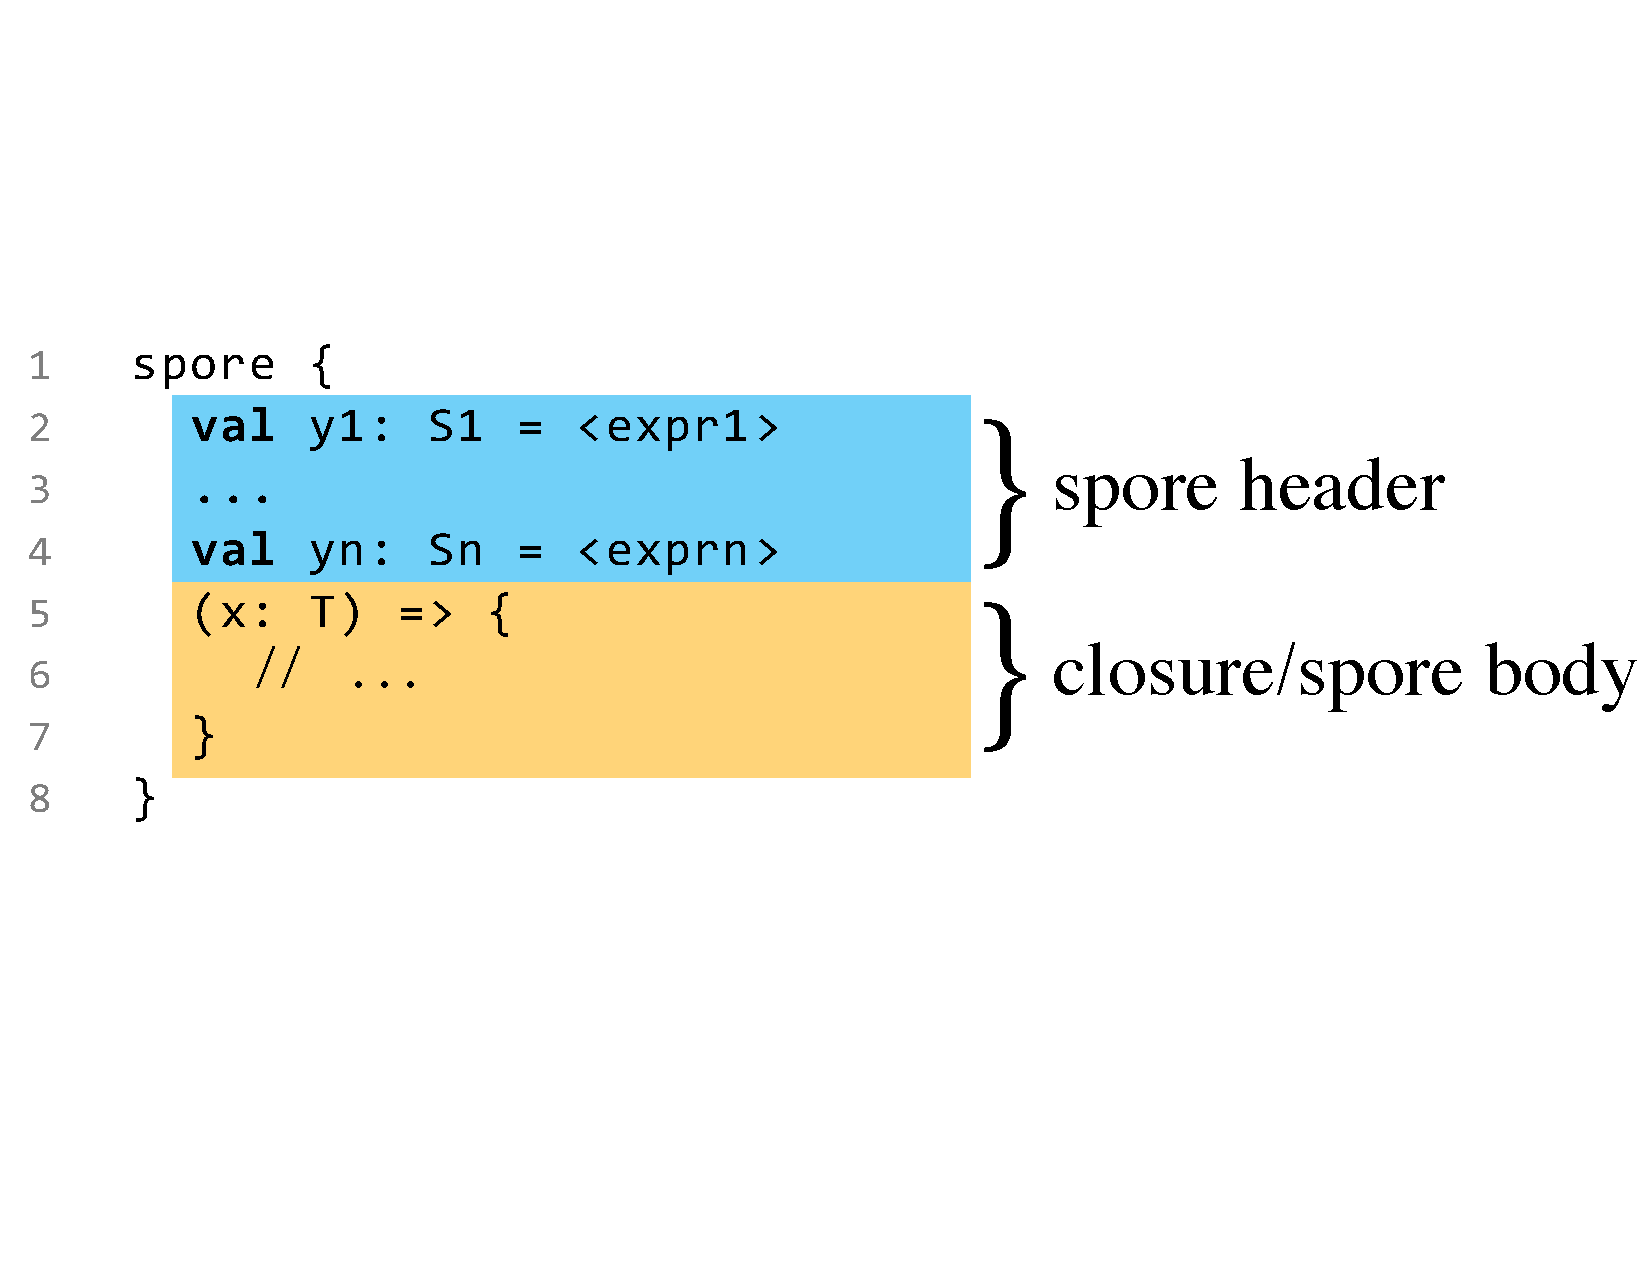
\includegraphics[width=7cm]{spore-shape.pdf}
\vspace{-0.4cm}
\caption{The syntactic shape of a spore.}
\label{fig:spore-shape}
\end{figure}
\setlength{\belowcaptionskip}{0pt}

A spore is a closure with a specific shape that dictates how the environment
of a spore is declared. The shape of a spore is shown in Figure~\ref{fig:spore-shape}.
A spore consists of two parts:
\vspace{-1.5mm}
\begin{itemize}
\item {\bf the spore header}, composed of a list of value definitions.
\item {\bf the spore body} (sometimes referred to as the ``spore closure''), a regular closure.
\end{itemize}

% The spore header is composed of a list of value definitions. The
% The list of value
% definitions at the beginning is called the spore header. The header is
% followed by a regular closure, the spore's body.

% \vspace{-1.5mm}
The characteristic property
of a spore is that the {\em spore body} is only allowed to access its
parameter, the values in the spore header, as well as top-level singleton objects
(public, global state). In particular, the spore closure is not allowed to
capture variables in the environment. Only an expression on the right-hand
side of a value definition in the spore header is allowed to capture
variables.

By enforcing this shape, the environment of a spore is always declared
explicitly in the spore header, which avoids accidentally capturing
problematic references -- such as unstable members (\eg method calls), mutable
fields, etc. Moreover, importantly for object-oriented langauges, it's no
longer possible to accidentally capture the \verb|this| reference.

% \setlength{\belowcaptionskip}{-4pt}
\begin{figure}%[b!]
\begin{subfigure}{.5\textwidth}
  \centering
  \begin{lstlisting}
  {
    val y1: S1 = <expr1>
    ...
    val yn: Sn = <exprn>
    (x: T) => {
      // ...
    }
  }
  \end{lstlisting}
  \caption{A closure block.}
  \label{fig:normal-block}
\end{subfigure}%
\begin{subfigure}{.5\textwidth}
  \centering
  \begin{lstlisting}
  spore {
    val y1: S1 = <expr1>
    ...
    val yn: Sn = <exprn>
    (x: T) => {
      // ...
    }
  }
  \end{lstlisting}
  \caption{A spore.}
  \label{fig:normal-spore-shape}
\end{subfigure}%
% \vspace{1mm}
\caption{The evaluation semantics of a spore is equivalent to that of a closure, obtained by simply leaving out the spore marker.}
\label{fig:evaluation-semantics}
\vspace{-5mm}
\end{figure}
% \setlength{\belowcaptionskip}{0pt}


\subsubsection{Evaluation Semantics}

Note that the evaluation semantics of a spore is equivalent to a closure
obtained by leaving out the \verb|spore| marker, shown in
Figure~\ref{fig:evaluation-semantics}.

In Scala, the block shown in Figure~\ref{fig:normal-block} first initializes
all value definitions in order and then evaluates to a closure that captures
the introduced local variables \verb|y1, ..., yn|. The corresponding spore,
shown in Figure~\ref{fig:normal-spore-shape} has the exact same evaluation
semantics. Interestingly, this closure shape is already used in production
systems such as Spark in an effort to avoid problems with accidentally
captured references, such as \verb|this|. However, in systems like Spark, the
above shape is merely a convention, it's not enforced, whereas with spores it
is.

\vspace{2mm}
\subsection{The \texttt{Spore} Type}
\label{sec:spore-type}
\vspace{1mm}

Like a normal function, the type of the \verb|spore| constructor contains the
spore closure's parameter type(s) as well as its return type. Unlike a normal function,
however, the \verb|Spore| type additionally contains information about
\textit{captured} and \textit{excluded} types. This information is represented
as (potentially abstract) \verb|Captured| and \verb|Excluded| type members of
the base \verb|Spore| type.

In general, individual spores are represented as {\em refinement types} of the
base \verb|Spore|, which, to be fully compatible with normal Scala functions,
is itself a subtype of one of Scala's function types.\footnote{This is possible, because in Scala functions are instances of classes that mix in one of the function traits.}
The type of a spore of arity-1, as well and Scala's arity-1 function type are
shown in Figure~\ref{fig:spore-type}.

\begin{figure}[b!]
\vspace{-2mm}
\begin{subfigure}{.5\textwidth}
  \centering
  \begin{lstlisting}
    trait Function1[-A, +B] {
      def apply(x: A):  B
    }
  \end{lstlisting}
  \caption{Scala's arity-1 function type.}
  \label{fig:function-arity1}
\end{subfigure}%
\begin{subfigure}{.5\textwidth}
  \centering
  \begin{lstlisting}
    trait Spore[-A, +B]
    extends Function1[A, B] {
      type Captured
      type Excluded
    }
  \end{lstlisting}
  \caption{The arity-1 \texttt{Spore} type.}
  \label{fig:spore-arity1}
\end{subfigure}%
\vspace{-1mm}
\caption{The \texttt{Spore} type.}
\label{fig:spore-type}
\vspace{-2mm}
\end{figure}

Figure~\ref{fig:function-arity1} show's Scala's arity-1 function type.\footnote{For simplicity, we omit definitions of the \verb+andThen+ and \verb+compose+ methods in the definition of \verb+Function1+.}
Here, the \verb|apply| method is abstract; a concrete implementation applies
the body of the function that's being defined to the argument \verb|x|.
Functions are contravariant in their argument type \verb|A|, indicated using
the \verb|-| symbol, and covariant in their result type \verb|B|, indicated
using the \verb|+| symbol.


% The result type of the \verb|spore| constructor is not a regular function type, but a subtype of one of Scala's function types. This is possible, because in Scala functions are instances of classes that mix in one of the function traits. For example, the trait for functions of arity one looks like this:

% \begin{lstlisting}
%     trait Function1[-A, +B] {
%       def apply(x: A):  B
%     }
% \end{lstlisting}

% \begin{lstlisting}
%     trait Spore[-A, +B] extends Function1[A, B] {
%       type Captured
%       type Excluded
%     }
% \end{lstlisting}


The \verb|Spore| type is shown in Figure~\ref{fig:spore-arity1}. Like normal
Scala functions, spores are contravariant in their argument type \verb|A|, and
covariant in their result type \verb|B|. Additionally, type \verb|Spore| has
two abstract type members. In a concrete spore, the \verb|Captured| type
member is defined to be a tuple type with the types of all captured variables.
We will introduce the \verb|Excluded| type member later, in Section~\ref{sec:excluded-types}

\vspace{2mm}
\subsection{Basic Usage}
\label{sec:basic-usage}
\vspace{1mm}

% simple spore (concrete example)
% for-comprehensions (example using that guy above)
% composition

\subsubsection{Definition}

A spore can be defined as shown in Figure~\ref{fig:captured-spore}, with its
corresponding type shown in Figure~\ref{fig:captured-type}. As can be seen,
the types of the environment listed in the spore header are
represented by the \verb|Captured| type member in the spore's type.

\begin{figure}[t!]
\begin{subfigure}{.5\textwidth}
  \centering
  \begin{lstlisting}
    val s = spore {
      val y1: String = expr1;
      val y2: Int = expr2;
      (x: Int) => y1 + y2 + x
    }
  \end{lstlisting}
  \caption{A spore \texttt{s} which captures a \texttt{String} and an \texttt{Int} in its spore header.}
  \label{fig:captured-spore}
\end{subfigure}%
\begin{subfigure}{.5\textwidth}
  \centering
  \begin{lstlisting}
    Spore[Int, String] {
      type Captured = (String, Int)
    }
  \end{lstlisting}
  \caption{\texttt{s}'s corresponding type.}
  \label{fig:captured-type}
\end{subfigure}%
\vspace{1mm}
\caption{An example of the \texttt{Captured} type member. \\\textit{Note: we omit the
\texttt{Excluded} type member for simplicity; we detail it later in Section~\ref{sec:excluded-types}.}}
\label{fig:captured-ex}
\vspace{-5mm}
\end{figure}

\subsubsection{Using Spores in APIs}

Spores can also be used in method definitions, for example, a method \verb|sendOverWire| can require arguments to be spores:

\begin{lstlisting}[numbers=none]
    def sendOverWire(s: Spore[Int, Int]): Unit = ...
\end{lstlisting}

\noindent Note that in this example, the \verb|Captured| (and \verb|Excluded|) type
member is not specified, meaning it is left abstract. In this case, so long as
the spore's parameter and result types match, a spore type is always
compatible, regardless of which types are captured.

Using spores in this way enables libraries and frameworks to enforce the use
of spores instead of plain closures, thereby reducing the risk for common
programming errors (see Section~\ref{sec:case-studies} for detailed case
studies), even in this very simple form. In later sections, we will see more
advanced ways in which library authors can control the capturing semantics of
a spore.

\subsubsection{Composition}

Like normal functions, spores can be composed. By representing the environment
of spores using refinement types, it is possible to preserve the captured type
information (and later, constraints) of spores when they are composed.

For example, assume we are given two spores \verb|s1| and \verb|s2| with types:

\begin{lstlisting}[numbers=none]
    s1: Spore[Int, String] { type Captured = (String, Int) }
    s2: Spore[String, Int] { type Captured = Nothing }
\end{lstlisting}

\noindent The fact that the \verb|Captured| type in \verb|s2| is defined to be
\verb|Nothing| means that the spore does not capture anything (\verb|Nothing|
is Scala's bottom type). The composition of \verb|s1| and \verb|s2|, written
\verb|s1 compose s2|, would therefore have the following refinement type:

\begin{lstlisting}[numbers=none]
    Spore[String, String] { type Captured = (String, Int) }
\end{lstlisting}

\noindent Note that the \verb|Captured| type member of the result spore is equal to the
\verb|Captured| type of \verb|s1|, since it is guaranteed that the result
spore does not capture more than what \verb|s1| already captures. Thus, not
only are spores composable, but so are their (refinement) types.

In Section~\ref{sec:adv-usage-type-constraints}, we'll see two kinds of ``type
constraints'' which provides more control over spore capturing semantics, and
thus the spore types, that our system provides, namely, {\em excluded types} and
{\em context bounds for captured types}. We will see that even with these added type constraints, the spore type is still composable.

\subsubsection{Implicitly Converting Functions to Spores}

The design of spores was guided in part by a desire to make them easy to use,
and easy to integrate in already closure-heavy code. Spores, as so far
proposed, introduce considerable verbosity in pursuit of the requirement to
explicitly define the spore's environment.

Therefore, it is also possible to use function literals as spores if they
satisfy the spore shape constraints. To support this, an implicit
conversion\footnote{In Scala, implicit conversions can be thought of as methods which can be implicitly invoked based upon their type, and whether or not they are present in implicit scope. Implicit conversions carry the \texttt{implicit} keyword before their declaration.}
macro\footnote{In Scala, macros are methods that are transparently loaded by the compiler and executed (or expanded) during compilation. A macro is defined like a normal method, but it is linked using the \texttt{macro} keyword to an additional method that operates on abstract syntax trees.} is provided which converts regular
functions to spores, but only if the converted function is a literal: only
then is it possible to enforce the spore shape.

\subsubsection{For-Comprehensions}

Converting functions to spores opens up the use of spores in a number of other
situations, most prominently, for-comprehensions\footnote{The implicit
conversion makes it possible to have for-comprehensions without altering the
Scala compiler, because de-sugaring the for-comprehension happens before
implicit conversions are inserted.} (Scala's version of Haskell's do-notation).
In Scala, for-comprehensions are desugared to invocations of the
higher-order \verb|map|, \verb|flatMap|, and \verb|filter|
methods, each of which take normal functions as arguments.

% \footnote{Lazy filtering is supported using the additional
% \verb|withFilter| method}

% The Scala specification contains the following rewrite rule:

%     A for-comprehension for (p <- e) yield e' is translated to e.map { case p => e' }

% Here, p is a general pattern expression, but is typically just a single-variable pattern (such as "i").

% Ideally, it should be possible that the map method used in the above translation requires its argument to be a spore. However,

% Since we'd like to avoid special treatment of spores within for-comprehensions, we'd like to rely on the above implicit conversion from functions to spores to enable this use case. Unfortunately, the shape of the functions generated by the desugaring of for-comprehensions is fixed; thus, it would be impossible for a generated function to capture anything, since there is no way to specify a spore header. This is however impractical, since capturing is unavoidable as soon as a for-comprehension has multiple generators:

%     for (a <- gen1; b <- gen2) yield a + b

% This is translated to:

%     gen1.flatMap(a => gen2.map(b => a + b))

In situations where for-comprehension closures capture variables, preventing
them from being converted implicitly to spores, we introduce an alternative
syntax for capturing variables in spores: an object that's referred to using a
so-called ``stable identifier'' \verb|id| can additionally be captured using
the syntax \verb|capture(id)|.\footnote{In Scala, a stable identifier is
basically a selection p.x where p is a path and x is an identifier (see Scala
Language Specification~\cite{ScalaSpec}, Section 3.1).}

This enables the use of spores in for-comprehensions, since it's possible to write:

\begin{lstlisting}[numbers=none]
    for (a <- gen1; b <- capture(gen2)) yield capture(a) + b
\end{lstlisting}

\noindent Note that superfluous \verb|capture| expressions are not harmful. Thus, it is
legal to write:

\begin{lstlisting}[numbers=none]
    for (a <- capture(gen1); b <- capture(gen2)) yield capture(a) + capture(b)
\end{lstlisting}

\noindent This allows the use of \verb|capture| in a way that does not require users to
know how for-comprehensions are desugared. In Section~\ref{sec:case-studies}
we show how capture and the implicit conversion of functions to spores enables
the use of for-comprehensions in the context of distributed programming with
spores.



% For example, the spore

% \begin{lstlisting}
%     spore { val y1: String = expr1; val y2: Int = expr2; (x: Int) => y1+y2+x }
% \end{lstlisting}

% would have the refinement type

% \begin{lstlisting}
%     Spore[Int, String] {
%       type Captured = (String, Int)
%     }
% \end{lstlisting}

\vspace{2mm}
\subsection{Advanced Usage and Type Constraints}
\label{sec:adv-usage-type-constraints}
\vspace{1mm}

In this section, we describe two different kinds of ``type constraints'' which
enable more fine-grained control over closure capture semantics; \emph{excluded
types} which prevent certain types from being captured, and \emph{context bounds} for
captured types which enforce certain type-based properties for all captured
variables of a spore. Importantly, all of these different kinds of constraints
compose, as we will see in later subsections.

% \todo{because these things are recorded in the type, they compose! That means that excluded types cannot be forgotten upon composition -- instead the resulting spore excludes the composition of the excluded types from the composed spores.}

Throughout this paper, we use as a motivating example hazards that arise in
concurrent or distributed settings. However, note that the system of type
constraints described henceforth is general, and can be applied to very
different applications and sets of types.

\subsubsection{Excluded Types}
\label{sec:excluded-types}

Libraries and frameworks for concurrent and distributed programming, such as Akka~\cite{Akka} and Spark, typically have requirements to avoid capturing certain types in closures that are used together with library-provided objects and methods. For example, when using Akka, one should not capture variables of type \verb|Actor|; in Spark, one should not capture variables of type \verb|SparkContext|.

Such restrictions can be expressed in our system by excluding types from being
captured by spores, using refinements of the \verb|Spore| type presented in
Section~\ref{sec:spore-type}. For example, the following refinement type
forbids capturing variables of type \verb|Actor|:

\begin{lstlisting}
type SporeNoActor[-A, +B] = Spore[A, B] {
  type Excluded <: No[Actor]
}
\end{lstlisting}
\noindent
Note the use of the auxiliary type constructor \verb|No| (defined as \lstinline{trait No[-T]}): it enables
the exclusion of multiple types while supporting desired sub-typing relationships.

% \begin{lstlisting}[numbers=none]
% trait No[-T]
% \end{lstlisting}
% \noindent

% (We explain the "-" annotation on the type parameter below when discussing sub-typing.)

\noindent For example, exclusion of multiple types can be expressed as follows:

\begin{lstlisting}
type SafeSpore = Spore[Int, String] {
  type Excluded = No[Actor] with No[Util]
}
\end{lstlisting}

\noindent Given Scala's sub-typing rules for refinement types, a spore refinement
excluding a superset of types excluded by an ``otherwise type-compatible''
spore is a subtype. For example, \verb|SafeSpore| is a subtype of
\verb|SporeNoActor[Int, String]|.

\paragraph{\textbf{\textit{Subtyping}}}

Using some frameworks typically user-defined subclasses are created that extend framework-provided types. However, the extended types are sometimes not safe to be captured. For example, in Akka, user-created closures should not capture variables of type \verb|Actor| and any subtypes thereof. To express such a constraint in our system we define the \verb|No| type constructor to be contravariant in its type parameter; this is the meaning of the \verb|-| annotation in the type declaration \verb|trait No[-T]|.

As a result, the following refinement type is a supertype of type\\
\verb|SporeNoActor[Int, Int]| defined above (we assume \verb|MyActor| is a subclass of \verb|Actor|):

\begin{lstlisting}
type MySpore = Spore[Int, Int] {
  type Excluded <: No[MyActor]
}
\end{lstlisting}
\noindent
It is important that \verb|MySpore| is a supertype and not a subtype of\\
\verb|SporeNoActor[Int, Int]|, since an instance of \verb|MySpore| could capture some other subclass of \verb|Actor| which is not itself a subclass of \verb|MyActor|. Thus, it would not be safe to use an instance of \verb|MySpore| where an instance of \verb|SporeNoActor[Int, Int]| is required. On the other hand, an instance of \verb|SporeNoActor[Int, Int]| is safe to use in place of an instance of \verb|MySpore|, since it is guaranteed not to capture \verb|Actor| or any of its subclasses.

\paragraph{\textbf{\textit{Reducing \texttt{Excluded} Boilerplate}}}

Given that the design of spores was guided in part by a desire to make them
easy to use, and easy to integrate in already closure-heavy code with minimal
changes, one might observe that the \verb|Spore| type with \verb|Excluded|
types introduces considerable verbosity. This is easily solved in practice by
the addition of a macro \verb|without[T]| which takes a type parameter
\verb|T| and rewrites the spore type to take into consideration the excluded
type \verb|T|. Thus, in the case of the \verb|SafeSpore| example, the same spore
refinement type can easily be synthesized inline in the definition of a spore value:

\begin{lstlisting}
val safeSpore = spore {
  val a = ...
  val b = ...
  (x: T) => { ... }
}.without[Actor].without[Util]
\end{lstlisting}

\subsubsection{Context Bounds for Captured Types}
\label{sec:context-bounds}
% \subsubsection{Attaching Properties with Context Bounds}

The fact that for spores a certain shape is enforced is very useful. However,
in some situations this is not enough. For example, a common source of race
conditions in data-parallel frameworks like Scala's parallel collections
manifests itself when users capture mutable objects (\eg an
instance of \verb|scala.collection.mutable.HashMap| from the Scala standard
library). Thus, a user might want to enforce that closures only capture
immutable objects. However, such constraints
cannot be enforced using the spore shape alone (captured objects are stored in
constant values in the spore header, but such constants might still refer to
mutable objects).

In this section, we introduce a form of type-based constraints called
``context bounds'' which enforce certain type-based properties for all
captured variables of that spore.\footnote{The name ``context bound'' is used
in Scala to refer to a particular kind of implicit parameter that is added
automatically if a type parameter has declared such a context bound. Our
proposal essentially adds context bounds to type members.}

Taking another example, it might be necessary for a spore to require the
availability of instances of a certain type class for the types of all of its
captured variables. A typical example for such a type class is \verb|Pickler|:
types with an instance of the \verb|Pickler| type class can be pickled using a
new type-based pickling framework for Scala~\cite{ScalaPickling}. To be able
to pickle a spore, it's necessary that all its captured types have an instance
of \verb|Pickler|.\footnote{A spore can be pickled by pickling its environment and
the fully-qualified class name of its corresponding function class.}

% because Property[T] allows requiring that all captured types implement the "interface" T
% and then you can continue like in the snippet you showed me about how it's not Java-style interfaces but more like JavaGI and C++...

Spores allow expressing such a requirement using a notion of implicit {\em
properties}. The idea is that if there is an implicit value\footnote{An implicit value is a value in \textit{implicit scope} that's statically selected based on its type.}
of type \verb|Property[Pickler]| in scope at the
point where a spore is created, then it is enforced that all captured types in
the spore header have an instance of the \verb|Pickler| type class
% \footnote{A type class is a combination of a generic trait and a set of implicit values that provide type-specialized implementations of that trait. It's an alternative for providing implementations of generic interfaces and a way to automatically dispatch to them.}:

\begin{lstlisting}
import spores.withPickler

spore {
  val name: String = <expr1>
  val age: Int = <expr2>
  (x: String) => { ...}
}
\end{lstlisting}
\noindent While an imported property does not have an impact on how a spore is
constructed (besides the property import), it has an impact on the result type
of the spore macro. In the above example, the result type would be a
refinement of the \verb|Spore| type:\footnote{In the code example, \texttt{implicitly[T]} returns the uniquely-defined implicit value of \texttt{T} which is in scope at the invocation site.}


\begin{lstlisting}
Spore[String, Int] {
  type Captured = (String, Int)
  implicit val ev$0 = implicitly[Pickler[Captured]]
}
\end{lstlisting}
\noindent For each property that's imported, the resulting spore refinement type
contains an implicit value with the corresponding type class instance for type
\verb|Captured|.

% Such implicit values allow retrieving a type class instance for the captured types of a given spore using Scala's implicitly function as follows:

% \begin{lstlisting}
%     val s = spore { ... }
%     implicitly[Pickler[s.Captured]]
% \end{lstlisting}

% Note that s.Captured is defined to be the type of the environment of spore s: a tuple with all types of captured variables.

\paragraph{\textbf{\textit{Expressing context bounds in APIs}}}

Using the above types and implicits, it's also possible for a method
to require argument spores to have certain context bounds. For example,
requiring argument spores to have picklers defined for their captured types
can be achieved as follows:

\begin{lstlisting}
def m[A, B](s: Spore[A, B])(implicit p: Pickler[s.Captured]) = {
  // ...
}
\end{lstlisting}


\subsubsection{Defining Custom Properties}

Properties can be introduced using the \verb|Property| trait (provided by the
spores library):

\begin{lstlisting}[numbers=none]
    trait Property[C[_]]
\end{lstlisting}
\noindent As a running example, we will be defining a custom  property for
immutable types. A custom property can be introduced using a generic trait,
and an implicit ``property'' object that mixes in the above \verb|Property|
trait:

\begin{lstlisting}
object safe {
  trait Immutable[T]
  implicit object immutableProp extends Property[Immutable]
  ...
}
\end{lstlisting}
\noindent
The next step is to mark selected types as immutable by defining an implicit object extending the desired list of types, each type wrapped in the \verb|Immutable| type constructor:

\begin{lstlisting}
object safe {
  ...
  import scala.collection.immutable.{Map, Set, Seq}
  implicit object collections extends Immutable[Map[_, _]] with
    Immutable[Set[_]] with Immutable[Seq[_]] with ...
}
\end{lstlisting}

\noindent
The above definitions allow us to create spores that are guaranteed to capture
only types \verb|T| for which an implicit of type \verb|Immutable[T]| exists.

It's also possible to define compound properties by mixing in multiple traits
into an implicit property object:

\begin{lstlisting}[numbers=none]
    implicit object myProps extends Property[Pickler] with Property[Immutable]
\end{lstlisting}
\noindent By making this compound property available in a scope within which spores are
created (for example, using an \verb|import|), it is enforced that those
spores have both the context bound \verb|Pickler| and the context bound
\verb|Immutable|.


\subsubsection{Composition}

Now that we've introduced type constraints in the form of excluded types and
context bounds, we present generalized composition rules for the types of
spores with such constraints.

To precisely describe the composition rules, we introduce the following
notation: the function $Excluded$ returns, for a given refinement type, the
set of types that are excluded; the function $Captured$ returns, for a given
refinement type, the set of types that are captured. Using these two
mathematical functions, we can precisely specify how the type members of the
resulting spore refinement type are computed. (We use the syntax $.type$
to refer to the singleton types of the argument spores and the result,
respectively.)

% \vspace{-5mm}
\begin{enumerate}

\item $Captured(res.type) = Captured(s1.type), Captured(s2.type)$

\item $Excluded(res.type) = \{ T \in Excluded(s1.type) \cup Excluded(s2.type) ~|~ T \notin Captured(s1.type) \cup Captured(s2.type) \}$

\end{enumerate}

The first rule expresses the fact that the sequence of captured types of the resulting refinement type is simply the concatenation of the captured types of the argument spores.

The second rule expresses the fact that the set of excluded types of the result refinement type is defined as the set of all types that are excluded by one of the argument spores, but that are not captured by any of the argument spores.

For example, assume two spores \verb|s1| and \verb|s2| with types:

\begin{figure}[h!]
\vspace{0.5mm}
\begin{subfigure}{.5\textwidth}
  \centering
  \begin{lstlisting}
Spore[Int, String] {
  type Captured = (Int, Util)
  type Excluded = No[Actor]
}
  \end{lstlisting}
  \vspace{-4mm}
  \caption{Type of spore \texttt{s1}.}
\end{subfigure}%
\begin{subfigure}{.5\textwidth}
  \centering
  \begin{lstlisting}
Spore[String, Int] {
  type Captured = (String, Int)
  type Excluded = No[Actor] with No[Util]
}
  \end{lstlisting}
  \vspace{-4mm}
  \caption{Type of spore \texttt{s2}.}
\end{subfigure}%
\label{fig:spore-composition}
\vspace{0.5mm}
\end{figure}

% \begin{lstlisting}
% Spore[Int, String] {
%   type Captured = (Int, Util)
%   type Excluded = No[Actor]
% }
% \end{lstlisting}
% \noindent
% and
% \begin{lstlisting}
% Spore[String, Int] {
%   type Captured = (String, Int)
%   type Excluded = No[Actor] with No[Util]
% }
% \end{lstlisting}

\noindent
The result of composing the two spores, \verb|s1 compose s2|, thus has the following type:

\begin{lstlisting}
Spore[String, String] {
  type Captured = (Int, Util, String, Int)
  type Excluded = No[Actor]
}
\end{lstlisting}

\paragraph{\textbf{Loosening constraints}}

Given that type constraints compose, it's evident that as spores compose, type
constraints can monotonically increase in number. Thus, it's important to note
that it's also possible to soundly loosen constraints using the regular type
widening rules.

Let's say we have a spore with the following (too elaborate) refinement type:

\begin{lstlisting}
val s2: Spore[String, Int] {
  type Captured = (String, Int)
  type Excluded = No[Actor] with No[Util]
}
\end{lstlisting}

\noindent
Then we can soundly drop constraints by assigning the spore to a variable or by passing it to a parameter of a supertype:

\begin{lstlisting}
type MySafeSpore = Spore[String, Int] {
  type Captured
  type Excluded <: No[Actor]
}
\end{lstlisting}

\begin{lstlisting}
val simpleSpore: MySafeSpore = s2

def m(s: Spore[String, Int] { type Excluded <: No[Actor] })

m(s2)
\end{lstlisting}



% =========== BEGINNING OF OLD SPORES SECTION ===========
% \section{Spores}

% Spores are a closure-like abstraction which aim to give users . They achieve this by (a) enforcing a
% specific syntactic shape which, and (b) adding a type system.

% We would like to constrain the environment of a spore to express properties
% such as:
% \begin{itemize}
% \item All captured objects must be serializable
% \item All captured objects must be thread-safe
% \item Captured objects must not be marked as unsafe for capturing
% \end{itemize}
% \noindent
% Such properties restrict the types of objects that a spore is allowed to
% capture. A naive way to achieve this would be to annotate certain types as
% ``not-safe-for-capturing''. However, this approach would be too inflexible,
% since some desirable properties are orthogonal to others. For example, a
% \verb|Promise| type~\cite{promise-paper} would be safe for capturing by a
% spore used in a concurrent setting, whereas it would not be safe for capturing
% by a spore that is intended to be serialized.

% Thus, rather than permitting or disallowing types to be captured, in our
% approach spores can express properties that the types of captured variables
% are required to have. For example, a spore might require all captured types to
% be thread-safe. Properties can also be composed, enabling spores to require
% their captured types to have multiple properties. For example, in addition to
% thread-safety, a spore may require its captured types to be serializable.
% (Such a spore would be well-suited for computations that should be executed
% concurrently on the same computer or on another computer depending on the
% current work load.)

% \subsection{The \texttt{Spore} trait}

% To express type constraints we leverage two features of Scala's type system.
% First, in Scala a function is an object of a type that extends one of the
% predefined function traits. Thus, it is possible to subclass the predefined
% function types. Second, in Scala classes and traits can be refined with value
% and type members. As we will see, type members are a natural way to express
% type constraints.

% The type of single-argument spores is defined as follows:

% \begin{lstlisting}
%     trait Spore[-A, +R] extends Function1[A, R] {
%       type Capture[T]
%     }
% \end{lstlisting}
% \noindent
% The \verb|Spore| trait extends the \verb|Function1| trait~\todo{variance annotations} which is defined as
% follows in Scala's standard library:

% \begin{lstlisting}
%     trait Function1[-A, +R] extends AnyRef {
%       def apply(v: A): R
%       def andThen[B](g: R => B): A => B
%       def compose[B](g: B => A): B => R
%     }
% \end{lstlisting}
% \noindent
% The above definition expresses the fact that functions are objects with an
% \verb|apply| method; function composition is supported using the
% \verb|andThen| and \verb|compose| methods.

% The \verb|Capture[T]| type member of the \verb|Spore| trait is used to express
% requirements of all captured types \verb|T| in the form of ``interfaces'' that
% the captured types \verb|T| have to implement. As we will see below, instead
% of using Java-style interfaces, we use a combination of traits and
% implicits~\cite{Oliveira2010} akin to generalized interfaces in
% JavaGI~\cite{WehrT11} or concepts in C++.

% For example, a spore from \verb|Int| to \verb|String| that requires all
% captured types to be serializable would have the following type:
% \begin{lstlisting}
%     Spore[Int, String] {
%       type Capture[T] = Pickler[T]
%     }
% \end{lstlisting}
% \noindent
% The type member \verb|Capture[T]| is defined such that for each captured type
% \verb|T| there must exist an instance of type \verb|Pickler[T]| (a ``pickler''
% that can serialize or pickle objects of type \verb|T|). Such instances are
% made available and looked up using Scala's {\em implicits} as shown below.

% Just like requiring all captured types to have a certain property, sometimes
% it's necessary to prevent types with a certain property from being captured.
% While in principle this could be supported by requiring a property that's not
% satisfied only by those types we wish to exclude from capturing, it would
% require declaring all types that are not excluded, which would lead to a lot
% of boilerplate. Instead, we introduce another type member \verb|NoCapture[T]|
% used to express properties that lead to rejection of a captured type:\todo{also discuss subtypes}

% \begin{lstlisting}
%     trait Spore[-A, +R] extends Function1[A, R] {
%       type Capture[T]
%       type NoCapture[T]
%     }
% \end{lstlisting}
% \noindent
% Given this way of introducing constraints it's even possible to require
% captured types to have multiple properties. Since properties are expressed
% using traits, properties can be combined using mix-in composition. For
% example, a spore requiring all captured types to be both serializable and
% thread-safe would look as follows:

% \begin{lstlisting}
%     Spore[Int, String] {
%       type Capture[T] = Pickler[T] with ThreadSafe[T]
%     }
% \end{lstlisting}
% \noindent
% The idea behind the property \verb|ThreadSafe| is that thread-safe types could
% provide dummy implementations of the interface \verb|ThreadSafe[T]|. Moreover,
% the \verb|with| keyword is used to create the mix-in composition of
% \verb|Pickler[T]| and \verb|ThreadSafe[T]|. This composition is guaranteed to
% be defined if we require all properties to be direct descendants of
% \verb|AnyRef|, the top type of all reference types in Scala.

% Spores without constraints have types of the following form:
% \begin{lstlisting}
%     Spore[A, R] {
%       type Capture[T] = NoConstraint[T]
%       type NoCapture[T] = NoConstraint[T]
%     }
% \end{lstlisting}

% \subsection{Library-specific constraints}

% One important goal of spores is to make the use of closure-based libraries
% safer. This is enabled through subtyping: instead of using regular function
% types, libraries can require the use of subtypes of the \verb|Spore| trait
% introduced above.

% For example, a concurrency library could declare certain types as not safe to
% be captured by closures. We can express this using a type class, say,
% \verb|Unsafe[T]|. For each type that should not be captured we introduce a
% type class instance. For example, the following implicit object introduces an
% instance of the \verb|Unsafe| type class for type \verb|Actor|:

% \begin{lstlisting}
%     implicit object unsafeActor extends Unsafe[Actor]
% \end{lstlisting}
% \noindent
% To ensure that closures never capture types that are declared in such a way as
% unsafe, the library could use the following type alias in place of the regular
% type for functions of arity one:

% \begin{lstlisting}
%     type SafeSpore[A, R] = Spore[A, R] {
%       type NoCapture[T] <: Unsafe[T]
%     }
% \end{lstlisting}
% \noindent
% The \verb|NoCapture| type member of the above \verb|Spore| subtype is refined
% with the {\em upper type bound} \verb|Unsafe[T]|. This ensures that only spore
% types whose \verb|NoCapture| type members mix in \verb|Unsafe| are compatible
% (of course, they could be even more restrictive).

% \subsection{Introducing custom constraints}

% \subsection{Composing spores}


% Type constraints for a newly defined spore can be introduced as follows:
% \begin{lstlisting}
%     spore {
%       val s: String = // ...
%       (p: Int) => {
%         (1 to p).map(x => s).mkString("-")
%       }
%     }.with[Pickler]
% \end{lstlisting}
% \noindent

% [explain how to exclude certain types]

% [ideally safety properties of types can be declared retro-actively.]

% [how do we motivate other, custom properties?]
%
% =========== END OF OLD SPORES SECTION ===========


% \section{Function-Passing Paradigm}

% Frameworks this new paradigm would enable. Relationship to NoSQL?

% \subsection{General Model}

% Goal of general model: to take this mess of closures and functions and trouble with environments that pains people across languages and propose an abstraction that gets rid of this confusion.

% Include in the general model typing rules that makes this abstraction guaranteeably shippable
% given some baseline simplified formalism.

% \subsection{Meat}

% Need to work out structure of this and an appropriate title for this section. Would include stuff like type system and type constraints for spores perhaps (or keep that in the general model section?). Composing spores with type constraints. Subtyping and type constraints.

% \subsubsection{OO}

% The question of -- I capture something of type MyActor
% and the spore forbids capturing type Actor, and MyActor <: Actor
% then what happens.

\section{Formalization}

% This section presents a formalization of our type system.

\label{sec:formal}

\begin{figure}[ht!]
  \centering

  $\ba[t]{l@{\hspace{2mm}}l}
t ::=     x                                 & \mbox{variable}
\\
\gap ~|~  (x: T) \Rightarrow t              & \mbox{abstraction}
\\
\gap ~|~  t~t                               & \mbox{application}
\\
\gap ~|~  \texttt{let}~x = t~\texttt{in}~t  & \mbox{let binding}
\\
\gap ~|~  \{ \seq{l = t} \}                 & \mbox{record construction}
\\
\gap ~|~  t.l                               & \mbox{selection}
\\
\gap ~|~  \texttt{spore}~\{~\seq{x : T = t}~; \seq{pn} ; (x: T) \Rightarrow t~\}  & \mbox{spore}
\\
\gap ~|~  \texttt{import}~pn~\texttt{in}~t  & \mbox{property import}
\\
\gap ~|~  t~\texttt{compose}~t              & \mbox{spore composition}
\\
 & \\
v ::=     (x: T) \Rightarrow t              & \mbox{abstraction}
\\
\gap ~|~  \{ \seq{l = v} \}                 & \mbox{record value}
\\
\gap ~|~  \texttt{spore}~\{~\seq{x : T = v}~; \seq{pn} ; (x: T) \Rightarrow t~\}  & \mbox{spore value}
\\
 & \\
T ::=     T \Rightarrow T                   & \mbox{function type} \\
\gap ~|~  \{ \seq{l : T} \}                 & \mbox{record type}   \\
\gap ~|~  \mathcal{S}                       & \mbox{}
\\
\mathcal{S} ::= T \Rightarrow T~\{~\texttt{type}~\mathcal{C} = \seq{T}~;~\seq{pn}~\}   & \mbox{spore type}
\\
\gap ~|~  T \Rightarrow T~\{~\texttt{type}~\mathcal{C}~;~\seq{pn}~\}   & \mbox{abstract spore type}
\\
P \in pn \rightarrow \mathcal{T} & \mbox {property map}
\\
\mathcal{T} \in \mathcal{P}(T)   & \mbox{type family}
%::= \epsilon & \mbox{type family} \\
%\gap ~|~ T, \mathcal{T} & \mbox{non-empty}\\
\\
 & \\
\Gamma ::=  \seq{x : T}          & \mbox{type environment}
\\
\Delta ::=  \seq{pn}             & \mbox{property environment}
\\
\ea$

  \caption{Core language syntax}
  \label{fig:syntax}
  % \vspace{-5mm}
\end{figure}


We formalize spores in the context of a standard, typed lambda calculus with records. Apart from novel language and type-systematic features, our formal development follows a well-known methodology~\cite{TAPL}. Figure~\ref{fig:syntax} shows the syntax of our core language. Terms are standard except for the \texttt{spore}, \texttt{import}, and \texttt{compose} terms. A \texttt{spore} term creates a new spore. It contains a list of variable definitions (the spore header), a list of property names, and the spore's closure. A property name refers to a type family (a set of types) that all captured types must belong to.

An illustrative example of a property name and its associated type family, but in the context of Scala, is a type class: a spore satisfies such a property if there is a type class instance for all its captured types.

An \texttt{import} term imports a property name into the property environment
within a lexical scope (a term); the property environment contains properties
that are registered as requirements whenever a spore is created. This is
explained in more detail in Section~\ref{sec:typing}. A \texttt{compose} term
is used to compose two spores. The core language provides spore composition as
a built-in feature, because type checking spore composition is markedly
different from type checking regular function composition (see
Section~\ref{sec:typing}).

The grammar of values is standard except for spore values; in a spore value each term on the right-hand side of a definition in the spore header is a value.

The grammar of types is standard except for spore types. Spore types are refinements of function types. They additionally contain a (possibly-empty) sequence of captured types, which can be left abstract, and a sequence of property names.

\subsection{Subtyping}\label{sec:subtyping}

Figure~\ref{fig:subtyping} shows the subtyping rules. Record (\textsc{S-Rec}) and function (\textsc{S-Fun}) subtyping are standard.

The subtyping rule for spores (\textsc{S-Spore}) is analogous to the subtyping rule for functions with respect to the argument and result types. Additionally, for two spore types to be in a subtyping relationship either their captured types have to be the same ($M_1 = M_2$) or the supertype must be an abstract spore type ($M_2 = \texttt{type}~\mathcal{C}$). The subtype must guarantee at least the properties of its supertype, or a superset thereof. Taken together, this rule expresses the fact that a spore type whose type member $\mathcal{C}$ is not abstract is compatible with an abstract spore type as long as it has a superset of the supertype's properties. This is important for spores used as first-class values: functions operating on spores with arbitrary environments can simply demand an abstract spore type. The way both the captured types and the properties are modeled corresponds to (but simplifies) the subtyping rule for refinement types in Scala (see Section~\ref{sec:adv-usage-type-constraints}).

Rule \textsc{S-SporeFun} expresses the fact that spore types are refinements of their corresponding function types, giving rise to a subtyping relationship.


\begin{figure*}[ht!]
  \centering

\begin{mathpar}
\inferrule[\textsc{S-Rec}]
{ \seq{l'} \subseteq \seq{l} \andalso l_i = l'_i \to T_i <: T'_i \land T'_i <: T_i
}
{ \{ \seq{l : T} \} <: \{ \seq{l' : T'} \}
}

\inferrule[\textsc{S-Fun}]
{ T_2 <: T_1 \andalso R_1 <: R_2
}
{ T_1 \Rightarrow R_1 <: T_2 \Rightarrow R_2
}

\inferrule[\textsc{S-Spore}]
{ T_2 <: T_1 \andalso R_1 <: R_2 \\
  \seq{pn'} \subseteq \seq{pn} \andalso M_1 = M_2 \lor M_2 = \texttt{type}~\mathcal{C}
}
{ T_1 \Rightarrow R_1~\{~M_1~;~\seq{pn}~\} <: T_2 \Rightarrow R_2~\{~M_2~;~\seq{pn'}~\}
}

\inferrule[\textsc{S-SporeFun}]
{ T_1 \Rightarrow R_1~\{~M~;~\seq{pn}~\} <: T_1 \Rightarrow R_1
}{}
\end{mathpar}
  \vspace{-5mm}
  \caption{Subtyping}
  \label{fig:subtyping}
  \vspace{-1mm}
\end{figure*}


\subsection{Typing rules}\label{sec:typing}

\begin{figure*}[ht!]
  \centering

\begin{mathpar}
\inferrule[\textsc{T-Var}]
{ x : T \in \Gamma
}
{ \Gamma ; \Delta \vdash x : T
}

% \vspace{0.4cm}

\inferrule[\textsc{T-Sub}]
{ \Gamma ; \Delta \vdash t : T'  \quad  T' <: T
}
{ \Gamma ; \Delta \vdash t : T
}

% \vspace{0.4cm}

\inferrule[\textsc{T-Abs}]
{ \Gamma, x : T_1 ; \Delta \vdash t : T_2
}
{ \Gamma ; \Delta \vdash (x: T_1) \Rightarrow t : T_1 \Rightarrow T_2
}

% \vspace{0.4cm}

\inferrule[\textsc{T-App}]
{ \Gamma ; \Delta \vdash t_1 : T_1 \Rightarrow T_2 \quad
  \Gamma ; \Delta \vdash t_2 : T_1
}
{ \Gamma ; \Delta \vdash (t_1~t_2) : T_2
}

% \vspace{0.4cm}

\inferrule[\textsc{T-Let}]
{ \Gamma ; \Delta \vdash t_1 : T_1 \quad \Gamma, x : T_1 ; \Delta \vdash t_2 : T_2
}
{ \Gamma ; \Delta \vdash \texttt{let}~x = t_1~\texttt{in}~t_2 : T_2
}

% \vspace{0.4cm}

\inferrule[\textsc{T-Rec}]
{ \Gamma ; \Delta \vdash \seq{t : T}
}
{ \Gamma ; \Delta \vdash \{ \seq{l = t} \} : \{ \seq{l : T} \}
}

% \vspace{0.4cm}

\inferrule[\textsc{T-Sel}]
{ \Gamma ; \Delta \vdash t : \{ \seq{l : T} \}
}
{ \Gamma ; \Delta \vdash t.l_i : T_i
}

% \vspace{0.4cm}

\inferrule[\textsc{T-Imp}]
{ \Gamma ; \Delta, pn \vdash t : T
}
{ \Gamma ; \Delta \vdash \texttt{import}~pn~\texttt{in}~t : T
}

% \vspace{0.4cm}

\inferrule[\textsc{T-Spore}]
{ \forall s_i \in \seq{s}.~\Gamma ; \Delta \vdash s_i : S_i \andalso
  \seq{y : S}, x : T_1 ; \Delta \vdash t_2 : T_2 \\
  \forall pn \in \Delta, \Delta'.~\seq{S} \subseteq P(pn)
}
{ \Gamma ; \Delta \vdash \texttt{spore}~\{~\seq{y : S = s}~; \Delta'; (x: T_1) \Rightarrow t_2~\} : \\
  T_1 \Rightarrow T_2~\{~\texttt{type}~\mathcal{C} = \seq{S}~;~\Delta, \Delta'~\}
}

% \vspace{0.4cm}

\inferrule[\textsc{T-Comp}]
{ \Gamma ; \Delta \vdash t_1 : T_1 \Rightarrow T_2~\{~\texttt{type}~\mathcal{C} = \seq{S}~;~\Delta_1~\} \\
  \Gamma ; \Delta \vdash t_2 : U_1 \Rightarrow T_1~\{~\texttt{type}~\mathcal{C} = \seq{R}~;~\Delta_2~\} \\
  \Delta' = \{ pn \in \Delta_1 \cup \Delta_2 ~|~ \seq{S} \subseteq P(pn) \land \seq{R} \subseteq P(pn) \}
}
{ \Gamma ; \Delta \vdash t_1~\texttt{compose}~t_2 : U_1 \Rightarrow T_2~\{~\texttt{type}~\mathcal{C} = \seq{S}, \seq{R}~;~\Delta'~\}
}

\end{mathpar}
  \caption{Typing rules}
  \label{fig:typing-rules}
  \vspace{-5mm}
\end{figure*}

Typing derivations use a judgement of the form $\Gamma ; \Delta \vdash t : T$. Besides the standard variable environment $\Gamma$ we use a property environment $\Delta$ which is a sequence of property names that are ``active'' while deriving the type $T$ of term $t$. The property environment is reminiscent of the implicit parameter context used in the original work on implicit parameters~\cite{LewisLMS00}; it is an environment for names whose definition sites ``just happen to be far removed from their usages.''

In the typing rules we assume the existence of a global property mapping $P$ from property names $pn$ to type families $\mathcal{T}$. This technique is reminiscent of the way some object-oriented core languages provide a global class table for type-checking. The main difference is that our core language does not include constructs to extend the global property map; such constructs are left out of the core language for simplicity, since the creation of properties is not essential to our model.

The typing rules are standard except for rules \textsc{T-Imp}, \textsc{T-Spore}, and \textsc{T-Comp}, which are new. Only these three type rules inspect or modify the property environment $\Delta$. Note that there is no rule for spore application, since there is a subtyping relationship between spores and functions (see Section~\ref{sec:subtyping}). Using the subsumption rule \textsc{T-Sub} spore application is expressed using the standard rule for function application (\textsc{T-App}).

Rule \textsc{T-Imp} imports a property $pn$ into the property environment within the scope defined by term $t$.

Rule \textsc{T-Spore} derives a type for a spore term. In the spore, all terms on right-hand sides of variable definitions in the spore header must be well-typed in the same environment $\Gamma ; \Delta$ according to their declared type. The body of the spore's closure, $t_2$, must be well-typed in an environment containing only the variables in the spore header and the closure's parameter, one of the central properties of spores. The last premise requires all captured types to satisfy both the properties in the current property environment, $\Delta$, as well as the properties listes in the spore term, $\Delta'$. Finally, the resulting spore type contains the argument and result types of the spore's closure, the sequence of captured types according to the spore header, and the concatenation of properties $\Delta$ and $\Delta'$. The intuition here is that properties in the environment have been explicitly imported by the user, thus indicating that all spores in the scope of the corresponding import should satisfy them.

Rule \textsc{T-Comp} derives a result type for the composition of two spores. It inspects the captured types of both spores ($\seq{S}$ and $\seq{R}$) to ensure that the properties of the resulting spore, $\Delta$, are satisfied by the captured variables of both spores. Otherwise, the argument and result types are analogous to regular function composition. Note that it's always possible to weaken the properties of a spore through spore subtyping and subsumption (\textsc{T-Sub}).

\subsection{Operational semantics}\label{sec:opsem}

\begin{figure*}[t!]
  \centering
\vspace{-14mm}
\begin{mathpar}
% \inferrule[\textsc{E-Let1}]
% { t_1 \rightarrow t'_1
% }
% { \texttt{let}~x = t_1~\texttt{in}~t_2 \rightarrow \texttt{let}~x = t'_1~\texttt{in}~t_2
% }


% \inferrule[\textsc{E-Let2}]
% { \texttt{let}~x = v_1~\texttt{in}~t_2 \rightarrow [x \mapsto v_1]t_2
% }{}

% \inferrule[\textsc{E-Rec}]
% { t_k \rightarrow t'_k
% }
% { \{ \seq{l = v}, l_k = t_k, \seq{l' = t'} \} \rightarrow \{ \seq{l = v}, l_k = t'_k, \seq{l' = t'} \}
% }

% \inferrule[\textsc{E-Sel1}]
% { t \rightarrow t'
% }
% { t.l \rightarrow t'.l
% }

% \inferrule[\textsc{E-Sel2}]
% { \{ \seq{l = v} \}.l_i \rightarrow v_i
% }{}

% \inferrule[\textsc{E-App1}]
% { t_1 \rightarrow t'_1
% }
% { t_1 t_2 \rightarrow t'_1 t_2
% }

% \inferrule[\textsc{E-App2}]
% { t_2 \rightarrow t'_2
% }
% { v_1 t_2 \rightarrow v_1 t'_2
% }

% \inferrule[\textsc{E-AppAbs}]
% { ((x : T) \Rightarrow  t) v \rightarrow [x \mapsto v]t
% }{}

\inferrule[\textsc{E-AppSpore}]
{ \forall pn \in \seq{pn}.~\seq{T} \subseteq P(pn)
}
{ \texttt{spore}~\{~\seq{x:T=v};\seq{pn};(x':T)\Rightarrow t~\}v' \rightarrow \seq{[x \mapsto v]}[x' \mapsto v']t
}

% \vspace{0.4cm}

\inferrule[\textsc{E-Spore}]
{ t_k \rightarrow t'_k
}
{ \texttt{spore}~\{~\seq{x : T = v}, x_k : T_k = t_k, \seq{x' : T' = t'}~; (x: T) \Rightarrow t~\} \rightarrow \\ \texttt{spore}~\{~\seq{x : T = v}, x_k : T_k = t'_k, \seq{x' : T' = t'}~; (x: T) \Rightarrow t~\}
}

\vspace{-0.3cm}

\inferrule[\textsc{E-Imp}]
{ \texttt{import}~pn~\texttt{in}~t \rightarrow insert(pn, t)
}{}

% \vspace{0.4cm}

\inferrule[\textsc{E-Comp1}]
{ t_1 \rightarrow t_1'
}
{ t_1~\texttt{compose}~t_2\rightarrow t_1'~\texttt{compose}~t_2
}

\vspace{-0.3cm}

\inferrule[\textsc{E-Comp2}]
{ t_2 \rightarrow t_2'
}
{ v_1~\texttt{compose}~t_2\rightarrow v_1~\texttt{compose}~t_2'
}

\vspace{-0.3cm}

\inferrule[\textsc{E-Comp3}]
{ \Delta = \{ p~|~p \in \seq{pn},\seq{qn}.~\seq{T} \subseteq P(p) \land \seq{S} \subseteq P(p)\}
}
{ \texttt{spore}~\{~\seq{x:T=v};\seq{pn};(x':T')\Rightarrow t~\}~\texttt{compose}~\texttt{spore}~\{~\seq{y:S=w};\seq{qn};(y':S')\Rightarrow t'~\} \rightarrow \\ \texttt{spore}~\{~\seq{x:T=v}, \seq{y:S=w} ; \Delta ; (y': S') \Rightarrow \texttt{let}~z' = t'~\texttt{in}~[x' \mapsto z']t\}
}
\end{mathpar}
  \vspace{-4mm}
  \caption[Operational Semantics]{Operational Semantics\footnotemark}
  \label{fig:opsem}
  \vspace{-7mm}
\end{figure*}

Figure~\ref{fig:opsem} shows the evaluation rules of a small-step operational semantics for our core language. The only non-standard rules are \textsc{E-AppSpore}, \textsc{E-Spore}, \textsc{E-Imp}, and \textsc{E-Comp3}. Rule \textsc{E-AppSpore} applies a spore literal to an argument value. The differences to regular function application (\textsc{E-AppAbs}) are (a) that the types in the spore header must satisfy the properties of the spore dynamically, and (b) that the variables in the spore header must be replaced by their values in the body of the spore's closure. Rule \textsc{E-Spore} is a simple congruence rule. Rule \textsc{E-Imp} is a computation rule that is always enabled. It adds property name $pn$ to all spore terms within the body $t$. The $insert$ helper function is defined in Figure~\ref{fig:helper} (we omit rules for \verb|compose| and \verb|let|, since they are analogous to rules \textsc{H-InsApp} and \textsc{H-InsSel}).

Rule \textsc{E-Comp3} is the computation rule for spore composition. Besides computing the composition in a way analogous to regular function composition, it defines the spore header of the result spore, as well as its properties. The properties of the result spore are restricted to those that are satisfied by the captured variables of both argument spores.

\footnotetext{For the sake of brevity, here we omit the standard evaluation rules. The complete set of evaluation rules can be found in the accompanying technical report~\cite{SporesFormally}}

\begin{figure*}[ht!]
  \centering
  \vspace{-1mm}
\begin{mathpar}

\inferrule[\textsc{H-InsSpore1}]
{ \forall t_i \in \seq{t}.~insert(pn, t_i) = t'_i \\
  insert(pn, t) = t'
}
{ insert(pn, \texttt{spore}~\{~\seq{x:T=t};\seq{pn};(x':T)\Rightarrow t~\}) = \\ \texttt{spore}~\{~\seq{x:T=t'};\seq{pn}, pn;(x':T)\Rightarrow t'~\}
}

% \vspace{0.4cm}

\inferrule[\textsc{H-InsSpore2}]
{ insert(pn, \texttt{spore}~\{~\seq{x:T=v};\seq{pn};(x':T)\Rightarrow t~\}) = \\
\texttt{spore}~\{~\seq{x:T=v};\seq{pn}, pn;(x':T)\Rightarrow t~\}
}{}

\vspace{-0.3cm}

\inferrule[\textsc{H-InsApp}]
{ insert(pn, t_1~t_2) = insert(pn, t_1)~insert(pn, t_2)
}{}

\inferrule[\textsc{H-InsSel}]
{ insert(pn, t.l) = insert(pn, t).l
}{}

\end{mathpar}
  \vspace{-0.6cm}
  \vspace{-2.5mm}
  \caption{Helper function $insert$}
  \label{fig:helper}
  \vspace{-5mm}
\end{figure*}

\subsection{Soundness}\label{sec:soundness}

This section presents a soundness proof of the spore type system. The proof is based on a pair of progress and preservation theorems~\cite{WrightF94}. A complete proof of soundness appears in the companion technical report~\cite{SporesFormally}. In addition to standard lemmas, such as Lemma~\ref{lem:substitution} and Lemma~\ref{lem:weak}, we also prove a lemma specific to our type system, namely Lemma~\ref{lem:pres-import}, which ensures types are preserved under property import. Soundness of the type system follows from Theorem~\ref{th:progress} and Theorem~\ref{th:pres}.

% \begin{lemma}
% \emph{(Canonical forms)}
% \label{lem:canonical}
% \begin{enumerate}

% \item If $v$ is a value of type $\{ \seq{l : T} \}$, then $v$ is $\{ \seq{l = v} \}$ where $\seq{v}$ is a sequence of values.

% \item If $v$ is a value of type $T \Rightarrow R$, then $v$ is either $(x: T_1) \Rightarrow t$ or \\ $\texttt{spore}~\{~\seq{y : S = v}~; \seq{pn} ; (x: T_1) \Rightarrow t~\}$ where $T <: T_1$ and $\seq{v}$ is a sequence of values.

% \item If $v$ is a value of type $T \Rightarrow R~\{~\texttt{type}~\mathcal{C} = \seq{S}~;~\seq{pn}~\}$, then $v$ is \\ $\texttt{spore}~\{~\seq{y : S = v}~; \seq{pn} ; (x: T_1) \Rightarrow t~\}$ where $T <: T_1$ and $\seq{v}$ is a sequence of values.

% % \item If $v$ is a value of type $T_1 \Rightarrow R_1~\{~\texttt{type}~\mathcal{C}~;~\seq{pn}~\}$, then $v$ is \\ $\texttt{spore}~\{~\seq{x : S = v}~; \seq{pn} ; (x: T_1) \Rightarrow t~\}$ where $\seq{v}$ is a sequence of values.

% \end{enumerate}
% \end{lemma}


\begin{theorem}
\emph{(Progress)}
\label{th:progress}
Suppose $t$ is a closed, well-typed term (that is, $\vdash t : T$ for some $T$). Then either $t$ is a value or else there is some $t'$ with $t \rightarrow t'$.
\vspace{-2.5mm}
\end{theorem}
\begin{proof}
By induction on a derivation of $\vdash t : T$. The only three interesting cases are the ones for spore creation, application (where we might apply a spore to some argument), and spore composition.
\end{proof}


\begin{lemma}
\emph{(Preservation of types under import)}
\label{lem:pres-import}
If $\Gamma ; \Delta, pn \vdash t : T$ then $\Gamma ; \Delta \vdash insert(pn, t) : T$
\vspace{-2.5mm}
\end{lemma}
\begin{proof}
By induction on a derivation of $\Gamma ; \Delta, pn \vdash t : T$.
\end{proof}


\begin{lemma}
\emph{(Preservation of types under substitution)}
\label{lem:substitution}
If $\Gamma, x : S ; \Delta \vdash t : T$ and $\Gamma ; \Delta \vdash s : S$, then $\Gamma ; \Delta \vdash [x \mapsto s]t : T$
\vspace{-2.5mm}
\end{lemma}
\begin{proof}
By induction on a derivation of $\Gamma, x : S ; \Delta \vdash t : T$.
\end{proof}


\begin{lemma}
\emph{(Weakening)}
\label{lem:weak}
If $\Gamma ; \Delta \vdash t : T$ and $x \notin dom(\Gamma)$, then $\Gamma, x : S ; \Delta \vdash t : T$.
\vspace{-2.5mm}
\end{lemma}
\begin{proof}
By induction on a derivation of $\Gamma ; \Delta \vdash t : T$.
\end{proof}


\begin{theorem}
\emph{(Preservation)}
\label{th:pres}
If $\Gamma ; \Delta \vdash t : T$ and $t \rightarrow t'$, then $\Gamma ; \Delta \vdash t' : T$.
\vspace{-2.5mm}
\end{theorem}
\begin{proof}
By induction on a derivation of $\Gamma ; \Delta \vdash t : T$.
\end{proof}


\subsection{Relation to spores in Scala}

The soundness proof (see Section~\ref{sec:soundness}) of the formal type system guarantees several important properties for well-typed programs which closely correspond to the pragmatic model of spores in Scala:

\begin{enumerate}

\item Application of spores: for each property name $pn$, it is ensured that the dynamic types of all captured variables are contained in the type family $pn$ maps to ($P(pn)$).

\item Dynamically, a spore only accesses its parameter and the variables in its header.

\item The properties computed for a composition of two spores is a safe approximation of the properties that are dynamically required.

\end{enumerate}


\subsection{Excluded types}

This section shows how the formal model can be extended with excluded types as described above (see Section~\ref{sec:adv-usage-type-constraints}). Figure~\ref{fig:syntax-ext} shows the syntax extensions: first, spore terms and values are augmented with a sequence of excluded types; second, spore types and abstract spore types get another member $\texttt{type}~\mathcal{E} = \seq{T}$ specifying the excluded types.

\vspace{2mm}
\begin{figure*}[ht!]
  \centering

  $\ba[t]{l@{\hspace{2mm}}l}
t ::=     ...                               & \mbox{terms}
\\
\gap ~|~  \texttt{spore}~\{~\seq{x : T = t}~; \seq{T}; \seq{pn} ; (x: T) \Rightarrow t~\}  & \mbox{spore}
\\
 & \\
v ::=     ...                               & \mbox{values}
\\
\gap ~|~  \texttt{spore}~\{~\seq{x : T = v}~; \seq{T}; \seq{pn} ; (x: T) \Rightarrow t~\}  & \mbox{spore value}
\\
 & \\
\mathcal{S} ::= T \Rightarrow T~\{~\texttt{type}~\mathcal{C} = \seq{T}~;~\texttt{type}~\mathcal{E} = \seq{T}~;~\seq{pn}~\}   & \mbox{spore type}
\\
\gap ~|~  T \Rightarrow T~\{~\texttt{type}~\mathcal{C}~;~\texttt{type}~\mathcal{E} = \seq{T}~;~\seq{pn}~\}   & \mbox{abstract spore type}
\\
\ea$

  \caption{Core language syntax extensions}
  \label{fig:syntax-ext}
  \vspace{-5mm}
\end{figure*}

Figure~\ref{fig:subtyping-ext} shows how the subtyping rules for spores have to be extended. Rule \textsc{S-ESpore} requires that for each excluded type $T'$ in the supertype, there must be an excluded type $T$ in the subtype such that $T' <: T$. This means that by excluding type $T$, subtypes like $T'$ are also prevented from being captured.


% \vspace{2mm}
\begin{figure*}[ht!]
  \centering
\begin{mathpar}

\inferrule[\textsc{S-ESpore}]
{ T_2 <: T_1 \andalso R_1 <: R_2 \\
  \seq{pn'} \subseteq \seq{pn} \andalso M_1 = M_2 \lor M_2 = \texttt{type}~\mathcal{C} \\
  \forall T' \in \seq{U'}.~\exists T \in \seq{U}.~T' <: T
}
{ T_1 \Rightarrow R_1~\{~M_1~;~\texttt{type}~\mathcal{E} = \seq{U}~;~\seq{pn}~\} \\ <: T_2 \Rightarrow R_2~\{~M_2~;~\texttt{type}~\mathcal{E} = \seq{U'}~;~\seq{pn'}~\}
}

\inferrule[\textsc{S-ESporeFun}]
{ T_1 \Rightarrow R_1~\{~M~;~E~;~\seq{pn}~\} <: T_1 \Rightarrow R_1
}{}

\end{mathpar}
  \vspace{-6mm}
  \caption{Subtyping extensions}
  \label{fig:subtyping-ext}
  \vspace{-2mm}
\end{figure*}
% \vspace{2mm}

Figure~\ref{fig:typing-ext} shows the extensions to the typing rules. Rule \textsc{T-ESpore} additionally requires that none of the captured types $\seq{S}$ is a subtype of one of the types contained in the excluded types $\seq{U}$. The excluded types are recorded in the type of the spore. Rule \textsc{T-EComp} computes a new set of excluded types $\seq{V}$ based on both the excluded types and the captured types of $t_1$ and $t_2$. Given that it is possible that one of the spores captures a type that is excluded in the other spore, the type of the result spore excludes only those types that are guaranteed not be captured.

% \vspace{2mm}
\begin{figure*}[ht!]
  \centering
\begin{mathpar}

\inferrule[\textsc{T-ESpore}]
{ \forall s_i \in \seq{s}.~\Gamma ; \Delta \vdash s_i : S_i \andalso
  \seq{y : S}, x : T_1 ; \Delta \vdash t_2 : T_2 \\
  \forall pn \in \Delta, \Delta'.~\seq{S} \subseteq P(pn) \andalso
  \forall S_i \in \seq{S}.~\forall U_j \in \seq{U}.~\lnot(S_i <: U_j)
}
{ \Gamma ; \Delta \vdash \texttt{spore}~\{~\seq{y : S = s}~; \seq{U}; \Delta'; (x: T_1) \Rightarrow t_2~\} : \\
  T_1 \Rightarrow T_2~\{~\texttt{type}~\mathcal{C} = \seq{S}~;~\texttt{type}~\mathcal{E} = \seq{U}~;~\Delta, \Delta'~\}
}

\inferrule[\textsc{T-EComp}]
{ \Gamma ; \Delta \vdash t_1 : T_1 \Rightarrow T_2~\{~\texttt{type}~\mathcal{C} = \seq{S}~;~\texttt{type}~\mathcal{E} = \seq{U}~;~\Delta_1~\} \\
  \Gamma ; \Delta \vdash t_2 : U_1 \Rightarrow T_1~\{~\texttt{type}~\mathcal{C} = \seq{R}~;~\texttt{type}~\mathcal{E} = \seq{U'}~;~\Delta_2~\} \\
  \Delta' = \{ pn \in \Delta_1 \cup \Delta_2 ~|~ \seq{S} \subseteq P(pn) \land \seq{R} \subseteq P(pn) \} \\
  \seq{V} = (\seq{U} \setminus \seq{R}) \cup (\seq{U'} \setminus \seq{S})
}
{ \Gamma ; \Delta \vdash t_1~\texttt{compose}~t_2 : U_1 \Rightarrow T_2~\{~\texttt{type}~\mathcal{C} = \seq{S}, \seq{R}~;~\texttt{type}~\mathcal{E} = \seq{V}~;~\Delta'~\}
}

\end{mathpar}
  \vspace{-4mm}
  \caption{Typing extensions}
  \label{fig:typing-ext}
  % \vspace{-5mm}
\end{figure*}
\vspace{2mm}

Figure~\ref{fig:opsem-ext} shows the extensions to the operational semantics. Rule \\ \textsc{E-EAppSpore} additionally requires that none of the captured types $\seq{T}$ are contained in the excluded types $\seq{U}$. Rule \textsc{E-EComp3} computes the set of excluded types of the result spore in the same way as in the corresponding type rule (\textsc{T-EComp}).

\begin{figure*}[ht!]
  \centering
\begin{mathpar}

\inferrule[\textsc{E-EAppSpore}]
{ \forall pn \in \seq{pn}.~\seq{T} \subseteq P(pn) \andalso
  \forall T_i \in \seq{T}.~T_i \notin \seq{U}
}
{ \texttt{spore}~\{~\seq{x:T=v}~;~\seq{U}~;~\seq{pn}~;~(x':T) \Rightarrow t~\}~v' \rightarrow \\ \seq{[x \mapsto v]}[x' \mapsto v']t
}

\vspace{0.4cm}

\inferrule[\textsc{E-EComp3}]
{ \Delta = \{ p~|~p \in \seq{pn},\seq{qn}.~\seq{T} \subseteq P(p) \land \seq{S} \subseteq P(p)\} \\
  \seq{V} = (\seq{U} \setminus \seq{S}) \cup (\seq{U'} \setminus \seq{T})
}
{ \texttt{spore}~\{~\seq{x:T=v}~;~\seq{U}~;~\seq{pn}~;~(x':T') \Rightarrow t~\}~\texttt{compose} \\ \texttt{spore}~\{~\seq{y:S=w}~;~\seq{U'}~;~\seq{qn}~;~(y':S') \Rightarrow t'~\} \rightarrow \\ \texttt{spore}~\{~\seq{x:T=v}, \seq{y:S=w}~;~\seq{V}~;~\Delta~; \\ (y': S') \Rightarrow \texttt{let}~z' = t'~\texttt{in}~[x' \mapsto z']t~\}
}
\end{mathpar}
  \vspace{-4mm}
  \caption{Operational semantics extensions}
  \label{fig:opsem-ext}
  \vspace{-5mm}
\end{figure*}



\section{Implementation}
\label{sec:implementation}

We have implemented spores as a macro library for Scala 2.10 and 2.11. Macros are an experimental feature introduced in Scala 2.10 that enable ``macro defs'', methods that take expression trees as arguments and that return an expression tree that is inlined at each invocation site of the macro. Macros are expanded during type checking in a way which enables macros to synthesize their result type during macro expansion, specialized for each expansion site.

The implementation for Scala 2.10 requires in addition a compiler plug-in that provides a backport of the support for Java 8 SAM types (``functional interfaces'') of Scala 2.11. SAM type support extends type inference for user-defined subclasses of Scala's standard function types which enables infering the types of spore parameters.

An expression \verb|spore { val y: S = s; (x: T) => /* body */ }| invokes the \verb|spore| macro which is passed the block \verb|{ val y... }| as an expression tree. A spore without type constraints simply checks that within the body of the spore's closure, only the parameter \verb|x| as well as the variables in the spore header are accessed according to the spore type-checking rules. The expression tree returned by the macro creates an instance of a {\em refinement type} of the abstract \verb|Spore| class that implements its \verb|apply| method (which itself is inherited from the corresponding standard Scala function trait) by applying the spore's closure. The \verb|Spore| class also has abstract type members \verb|Captured| and \verb|Excluded|. The \verb|Captured| type member is defined by the generated refinement type to be a tuple type with the types of all captured variables. If there are no type constraints the \verb|Excluded| type member is defined to be \verb|No[Nothing]|.

Type constraints are implemented as follows. First, invoking the generic \verb|without| macro passing a type argument \verb|T|, say, augments the generated \verb|Spore| refinement type by effectivly adding the clause \verb|with No[T]| to the definition of its \verb|Excluded| type member. Second, the existence of additional bounds on the captured types is detected by attempting to infer an implicit value of type \verb|Property[_]|. If such an implicit value can be inferred, a sequence of types specifying type bounds is obtained as follows. Basically, the type of the implicit value is matched against the pattern \\ \verb|Property[t1] with ... with Property[tn]| where the \verb|ti| are type variables. For each type \verb|ti| an implicit value member

\begin{lstlisting}[numbers=none]
    implicit val evi: ti[Captured] = implicitly[ti[Captured]]
\end{lstlisting}
\noindent
is generated and added to the \verb|Spore| refinement type.

We also provide an implicit conversion from standard Scala functions to spores. This conversion is implemented as a macro whose expansion fails if the argument function is not a literal, since in this case it is impossible for the macro to check the spore shape/capturing constraints.

% Comparison and relationship with Java8 SAM stuff. Cite paper {\em Java SAM Typed Closures: A Sound and Complete Type Inference System for Nominal Types} ~\cite{JavaSAM}


\section{Evaluation}
\label{sec:evaluation}



% program        | LOC | #closures | #converted | LOC changed | #captured vars
%
% funsets        |  99 | 8         | 8          | 7           | 9
% forcomp        | 201 | 6         | 4          | 4           | 0
% mandelbrot     | 325 | 1         | 1          | 9           | 6
% barneshut      | 722 | 7         | 7          | 8           | 1
% spark pagerank |  64 | 5         | 5          | 8           | 0
% spark kmeans   |  92 | 5         | 4          | 9           | 2

% total          |1503 | 32        | 29         | 45          | 18

% pagerank   | ??  | ??        | ??         | ??          | ??

% \begin{figure*}
% % \onecolumn
% % \setlength\LTleft{10pt}            % default: \parindent
% % \setlength\LTright{10pt}           % default: \fill
% \begin{longtable}{l c@{}c c@{}c c@{}c c@{}c c@{}c }
% \toprule%

% {\bfseries Program} && {\bfseries LOC} && {\bfseries \#closures} && {\bfseries \#converted} && {\bfseries LOC changed} && {\bfseries \#captured vars} \\

% \cmidrule(l){0-1} \cmidrule(l){2-3} \cmidrule(l){4-5} \cmidrule(l){6-7} \cmidrule(l){8-9} \cmidrule(l){10-11} %\cmidrule(l){12-13}

% % \endhead


% funsets && 99 && 8 && 8 && 7 && 9 \\

% \myrowcolour%
% forcomp && 201 && 6 && 4 && 4 && 0 \\

% mandelbrot && 325 && 1 && 1 && 9 && 6 \\

% \myrowcolour%
% barneshut && 722 && 7 && 7 && 8 && 1 \\

% spark pagerank && 64 && 5 && 5 && 8 && 0 \\

% \myrowcolour%
% spark kmeans && 92 && 5 && 4 && 9 && 2 \\

% \bottomrule

% \textbf{Total} && 1503 && 32 && 29 && 45 && 18 \\

% \bottomrule

% \end{longtable}
% \caption{Comparison to related approaches}
% % \twocolumn
% \end{figure*}

In this section we evaluate the practicality and the benefits of using spores
as an alternative to normal closures in Scala. The evaluation has three parts.
In the first part we measure the impact of introducing spores in existing
programs. In the second part we evaluate the importance of excluding specific
types from the environment of closures. In the third part we evaluate the
syntactic overhead of spores in a large code base of big data-style
applications.

\subsection{Using Spores Instead of Closures}

In this section we measure the number of changes required to convert existing
programs that crucially rely on closures to use spores. We analyze a number of
real Scala programs, taken from three categories:
\begin{enumerate}
\vspace{-1mm}
\item General, closure-heavy code, taken from the exercises of the popular MOOC on Functional Programming Principles in Scala; the goal of analyzing this code is to get an approximation of the worst-case effort required when consistently using spores instead of closures, in a mostly-functional code base.

\item Parallel applications based on Scala's parallel collections. These examples evaluate the practicality of introducing spores into a parallel code base to increase its robustness.

\item Distributed applications based on the Apache Spark cluster computing framework. In this case, we evaluate the practicality of using spores in Spark applications to make sure closures are guaranteed to be serializable.
\vspace{-2mm}
\end{enumerate}

\begin{figure}[t!]
\centering
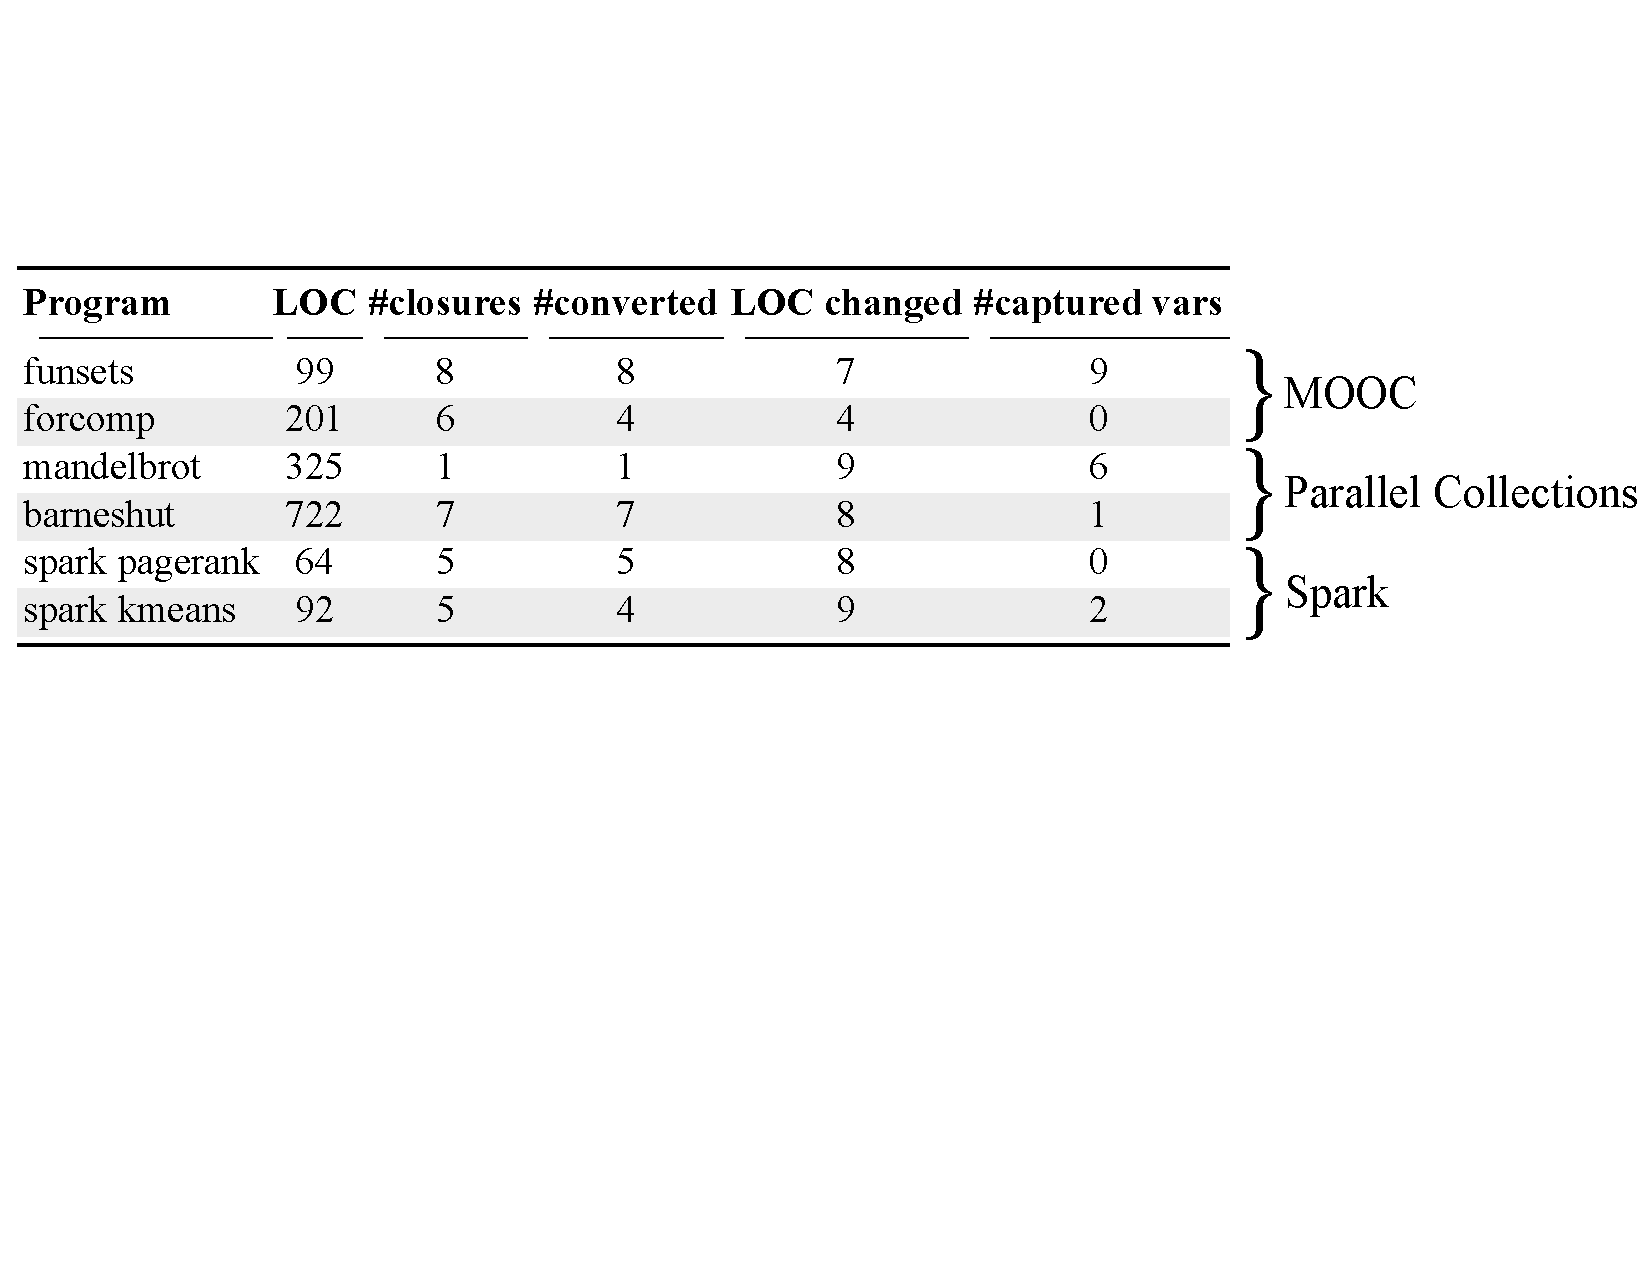
\includegraphics[width=\textwidth]{evaluation.pdf}
\caption{Evaluating the practicality of using spores in place of normal closures}
\label{fig:spore-eval}
\vspace{-5mm}
\end{figure}

\paragraph{\textbf{Methodology}} For each program, we obtained (a) the number of closures in the program that are candidates for conversion, (b) the number of closures that could be converted to spores, (c) the changed/added number of LOC, and (d) the number of captured variables. It is important to note that during the conversion it was not possible to rely on an implicit conversion of functions to spores, since the expected types of all library methods that were invoked by the evaluated applications remained normal function types (\ie they were not converted to spore types); thus, the reported numbers are worse than they would be for APIs using spores.

\paragraph{\textbf{Results}} The results are shown in Figure~\ref{fig:spore-eval}. Out of 32 closures 29 could be converted to spores with little effort. One closure failed to infer its parameter type when expressed as a spore. Two other closures could not be converted due to implementation restrictions of our current prototype. On average, per converted closure 1.4 LOC had to be changed. This number is dominated by two factors: the inability to use the implicit conversion from normal functions to spores, and one particularly complex closure in ``mandelbrot'' that required changing 9 LOC. In our programs, the number of captured variables is on average 0.56. These results suggest that programs using closures in non-trivial ways can typically be converted to using spores with relatively little effort, even if the used APIs do not use spore types.


\section{Case Studies}
\label{sec:case-studies}

\subsection{More Robust Distribution of Closures}

Frameworks like MapReduce~\cite{MapReduce} and Apache Spark~\cite{Spark} are designed for processing large datasets in a cluster. The programming models of these frameworks rely on distributing functions used for well-known map/reduce computation patterns.

In Spark, these patterns are directly expressed in Scala using the standard higher-order functions \verb|map| and \verb|reduce| applied to an abstraction for distributed collections called ``resilient distributed dataset'' (RDD). However, to avoid unexpected runtime exceptions due to unserializable closures when passing closures to RDDs, programmers must adopt conventions that are subtle and unchecked by the Scala compiler.

The following example shows a typical pattern extracted from a code base used in production:

\begin{lstlisting}
class GenericOp(sc: SparkContext, mapping: Map[String, String]) {
  private var cachedSessions: spark.RDD[Session] = ...

  def doOp(keyList: List[...], ...): Result = {
    val localMapping = mapping

    val mapFun: Session => (List[String], GenericOpAggregator) = { s =>
      (keyList, new GenericOpAggregator(s, localMapping))
    }

    val reduceFun: (GenericOpAggregator, GenericOpAggregator) =>
      GenericOpAggregator = { (a, b) => a.merge(b) }

    cachedSessions.map(mapFun).reduceByKey(reduceFun).collectAsMap
  }
}
\end{lstlisting}
\noindent
The \verb|GenericOp| class provides a method \verb|doOp| which performs a compound operation on the RDD \verb|cachedSessions|. \verb|GenericOp| has a parameter of type \verb|SparkContext|, the main entry point for functionality provided by Spark, and a parameter of type \verb|Map[String, String]| used within \verb|doOp|. The main computation of \verb|doOp| is the last expression of its body: a chain of invocations of \verb|map|, \verb|reduceByKey|, and \verb|collectAsMap|. To ensure that the argument closures of \verb|map| and \verb|reduceByKey| are serializable, the code follows two conventions: first, instead of defining \verb|mapFun| and \verb|reduceFun| as methods of class \verb|GenericOp|, they are defined using lambdas stored in local variables. Second, instead of using the \verb|mapping| parameter directly, it is first copied into a local variable \verb|localMapping|. The reason for the first convention is that in Scala converting a method to a function implicitly captures a reference to the enclosing object. However, \verb|GenericOp| is not serializable, since it refers to a \verb|SparkContext| which is not serializable. The reason for the second convention is that using \verb|mapping| directly, would result in \verb|mapFun| capturing the \verb|this| reference to be able to access it.

\subsubsection{Applying Spores}

Using spores, the above conventions can be enforced by the compiler, avoiding unexpected runtime exceptions. It is sufficient to turn \verb|mapFun| and \verb|reduceFun| into spores:

\begin{lstlisting}
val mapFun: Spore[Session, (List[String], GenericOpAggregator)] =
  spore { val localMapping = mapping
    (s: Session) => (keyList, new GenericOpAggregator(s, localMapping)) }

val reduceFun: Spore[(GenericOpAggregator, GenericOpAggregator),
                      GenericOpAggregator] =
  spore { (a, b) => a.merge(b) }
\end{lstlisting}
\noindent
The spore shape enforces the use of \verb|localMapping| (moved from the method body into \verb|mapFun|). Furthermore, there is no more possibility of accidentally capturing a reference to the enclosing object.


\subsection{Safer Closures for Parallel Collections}

Scala's parallel collections provide data-parallel operations for standard collection types like maps and sequences. These data-parallel operations typically take closures as arguments that are applied to all elements of the underlying collection in parallel. Unfortunately, it is easy to create race conditions by capturing mutable objects within such closures, and Scala's type checker does not provide any assistance for avoiding them.

Spores with context bounds allow making the use of parallel collections safer by preventing mutable objects from being captured in closures passed to data-parallel operations. In the following we show how this can be achieved using the custom property for immutable types shown in Section~\ref{sec:adv-usage-type-constraints} as well as a wrapper API utilizing spores instead of regular closures.

To ensure that only spores with context bound \verb|Immutable| are passed to data-parallel, higher-order methods such as \verb|map|, we provide a wrapper for \verb|ParIterable[A]|, the supertype of all parallel collections:

\begin{lstlisting}
class ImmutWrapper[A](parcoll: ParIterable[A]) {
  def map[B](s: Spore[A, B])(implicit i: Immutable[s.Captured]) =
    new ImmutWrapper(parcoll.map(s))
}
\end{lstlisting}
\noindent
Thanks to the implicit parameter, an invocation of \verb|map| only type-checks if an implicit of type \verb|Immutable[s.Captured]| is in scope; this is the case, if there is an implicit value of type \verb|Immutable[T]| in scope for each captured type \verb|T| of spore \verb|s|. This wrapper is then used as follows (assuming an \verb|import safe.{immutableProp, collections}|):

\begin{lstlisting}
val m: Map[Int, String] = ...
val pcoll = myColl.par
(new ImmutWrapper(pcoll)).map { elem =>
  if (m.apply(elem)) transform1(elem)  // OK, m is immutable!
  else transform2(elem)
}
\end{lstlisting}
\noindent
In the above example, capturing a mutable object (or, in fact, any object of type \verb|T| that does not have an implicit value of type \verb|Immutable[T]|) would lead to a compile-time error, thus preventing a potential data race.

% \section{Use-Cases?}

% We could show in an example-driven (or even paradigm-driven) way how the
% active objects pattern can be implemented on top of spores. And then we can
% show how spores help enforce certain safety properties that are important for
% that pattern. For example, in the active objects pattern it's important to
% either capture only immutable things, or clone things upon capturing.

% Paradigms or patterns built on top of spores:

% \begin{itemize}
% \item Distributed collections like Spark
% \item Active objects
% \item Futures
% \item Hot-swapping actors
% \item Distributed pipelines / distributed streams
% \end{itemize}

\section{Other Related Work}
\label{sec:related-work}

Parallel closures~\cite{ParallelClosures} are a variation of closures that make data in the environment available using read-only references using a type system for reference immutability. This enables parallel execution without the possibility of data races. Spores are not limited to immutable environments, and do not require a type system extension. River Trail~\cite{HerhutHSS13} provides a concurrency model for JavaScript, similar to parallel closures; however, capturing variables in closures in currently not supported.

HdpH~\cite{HDPH} generalizes Cloud Haskell's closures in several aspects: first, closures can be transformed without eliminating them. Second, unnecessary serialization is avoided, e.g., when applying a closure immediately after creation. Otherwise, the discussion of Cloud Haskell in Section~\ref{sec:sel-rel-work} also applies to HdpH. Delimited continuations~\cite{DelimitedContinuations} represent a way to serialize behavior in Scala, but don't resolve any of the problems of normal Scala closures when it comes to accidental capture, as spores do.

Termite Scheme~\cite{Termite} is a Scheme dialect for distributed programming based on an Erlang-style concurrency model. Closures and continuations are always serializable, since references to non-serializable objects (like open files or physical devices) are automatically wrapped in processes that are serialized as their process ID. In contrast, with spores there is no such automatic wrapping. Unlike closures in Termite Scheme, spores are statically-typed, supporting type-based constraints. Distributed Functional Programming in Scheme~\cite{DFPS} also provides serializable closures in a dynamically-typed setting. Python's standard serialization module, \verb|pickle|, does not support serializing closures. Dill~\cite{dill} extends Python's \verb|pickle| module, adding support for functions and closures. Constraints are not supported.


% Java RMI~\cite{JavaRMI}


% Supporting imperative features typically requires complex effect systems~\cite{DPJ}. our paper provides simpler ways to make programming with closures in imperative OO languages safer
% Lighter-weight alternative approach to some kind of crazy type and effect system.

% Should reference Cloud Types~\cite{CloudTypes}



\section{Conclusion}
\label{sec:conclusion}

We've presented a type-based foundation for closures, called spores, designed
to avoid various hazards that arise particularly in concurrent or distributed
settings. We have presented a flexible type system for spores which enables
composability of differently-constrained spores as well as custom user-defined
type constraints. We formalize and present a full soundness proof, as well as
an implementation of our approach in Scala.

A key takeaway of our approach is that including type information of captured
variables in the type of the spore enables a number of previously impossible
opportunities, including but not limited to controlled capture in concurrent,
distributed, and other arbitrary scenarios where closures must be
controlled.

Finally, we demonstrate the practicality of our approach through a small
empirical study, and show that converting non-trivial
programs to use spores requires relatively little effort. We also illustrate
the benefits of spores with and without type constraints in several real-world
case studies.



% through examples and case studies, we have shown the

% A key takeaway is that it enables a bunch of goodies for distributed and concurrent programming.
% But it also.

% key ideas are this.
% proven soundness.

% We've demonstrated its practicality through a small empirical study, using spores even without all of the automatic conversions isn't that intrusive for all of the safety it offers.
% We've illustrated the benefits of the safety guarantees of spores for several real-world use-cases. (custom type constraints)
% validated many design principles through evaluation and case studies
% Play up this everything being in the spore type point, and what enables in the intro and abstract.

% Spores should be able to express type-based
% properties of captured variables in a statically safe way. Including type
% information of captured variables in the type of a spore creates a number of
% previously impossible opportunities; it facilitates the verification of
% closure-heavy code; it opens up the possibility for IDEs to assist in safe
% closure creation, advanced refactoring, and debugging support; it enables
% compilers to implement safe transformations that can further simplify the use
% of safe closures, and it makes it possible for spores to integrate with type
% class-based frameworks like Scala/pickling~\cite{ScalaPickling}.


\bibliographystyle{abbrv}
\bibliography{bib}

\end{document}